
Whether developers co-evolve their code either manually or automatically, they cannot ensure that the code co-evolution is behaviorally correct, i.e., without altering the behavior of their impacted code. Especially, when there is other alternative co-evolutions for the same impacted code (challenge \Circled{\hyperref[C2]{C2}}). 
One way to check this is to re-run all the tests after each code co-evolution, which is expensive and time-consuming. It is also tedious and error-prone when the developer checks the output of the tests' execution and manually maps them between the original and evolved versions.
% Whereas several existing approaches automate the metamodels and code co-evolution  refs 

This chapter presents a new fully automatic approach to check the behavioral correctness of the code co-evolution between different releases of a language when its metamodel evolves. This approach leverages the test suites of the original and evolved versions of the language, and hence, its metamodels and code. 
%Test suites are usually used to check the code is behaviorally correct. 

Section~\ref{sec_background} presents the key concepts as a background followed by a motivation example. 
In section~\ref{sec_approach}, I detail the approach for testing metamodel and code co-evolution and how I use unit test suites before and after code co-evolution to check that the co-evolution did not alter the behavior of the code, while Section~\ref{sec_evaluation} evaluates it. The evaluation section presents first our user study experiment to gain evidence on the difficulty or not of the manual task of tracing impacted tests after metamodel evolution and co-evolution. Then, I measured the efficiency of this approach and the gains observed compared to using the whole test suite as a baseline.
Sections~\ref{threat} discusses internal and external threats to validity. 
Finally, Section~\ref{sec_conclusion} concludes the chapter. 
%In this approach, I use unit test suites before and after code co-evolution to check that the co-evolution did not alter the behavior of the code. % 
%The approach first takes as input the metamodel evolution changes and then parses the code to compute the code call graph (CCG). With the changes and the CCG, \red{we first locate all usages of the metamodel elements in the generated code. For example, a getter/setter of a metamodel attribute/reference, interface, the class implementation, etc. 
%	After that, we recursively trace the code usages of the metamodel elements in the CCG throughout the methods calls in the addition8813263al code until reaching the test methods.}
%Thus, we end up matching the metamodel changes with impacted code methods and their corresponding tests. We perform this step on both releases corresponding to the original and evolved metamodels and code to be able to check the behavioral correctness of the code before and after co-evolution.  
%
%We implemented our approach in an Eclipse plugin that allows to trace the tests, map them with state-of-the-art solution GumTree \cite{falleri2014fine} and execute them. Then, we report them back in a form of diagnostic to the developers for an easier in-depth analysis of the effect of metamodel evolution rather than re-running and analyzing the whole test suite.


%A first part of the evaluation consisted of an user study experiment to gain evidence on the difficulty or not of the manual task of tracing impacted tests after metamodel evolution and co-evolution. We found that tracing manually the tests impacted by the evolution of the metamodel is a hard and error-prone task. Not only the participants could not trace all tests, but they even wrongly traced non-impacted tests. The post-questionnaire results after a demonstration of our automatic approach suggest its high usefulness and adoption likelihood. 
%
%We then evaluated our approach on 18 Eclipse projects from OCL, Modisco, Papyrus, and EMF over several evolved versions of metamodels.  

%Section 1 presents ...


\section{Background and Example}
\label{sec_background}




This section gives a background on how metamodels play a significant role when building software languages and their tooling for a better comprehension of the current work. It then discusses the scenario of co-evolution that arises between metamodels and code, and the need for testing its behavioral correctness. 

\begin{figure*}[tb]
	\centering
	%\hspace*{-1em}
	% \vspace{-5mm}
	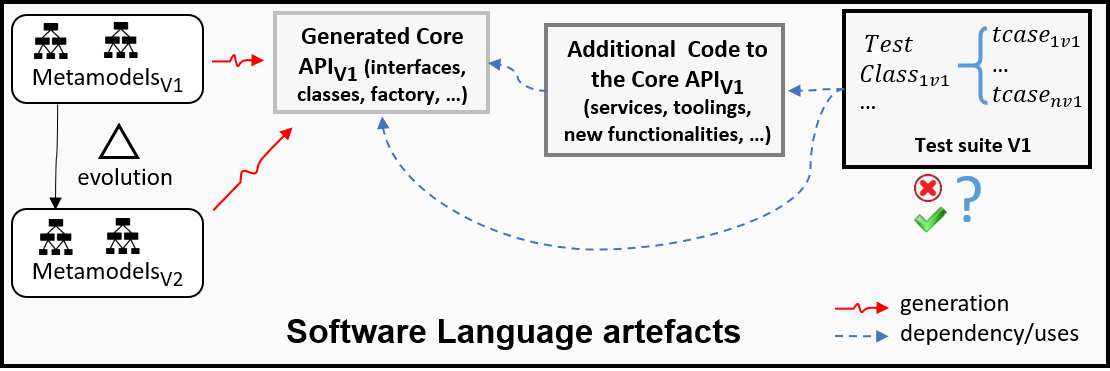
\includegraphics[width=0.9\textwidth]{./pics/chapter2pics/background.png}
	%\caption{Artifacts and structure of a software language in the Eclipse platform.}
	\caption{Evolution of metamodels and related artifacts of a software language}
	\label{fig:SL_useage}
	%\vspace{-5mm}
\end{figure*}


\subsection{Key Concepts}

%\red{Metamodels are a cornerstone in MDE. It serves to create model instances, constraints, or transformations. 
%	In our work, we focus on the relation between metamodels and code.
%}  
%
%Metamodels are cornerstones when building a software language and its toolings \cite{van2000domain,gronback2009eclipse}. 
%Metamodels define the aspects of a business domain, i.e. the main concepts, their properties, and relationships between them \cite{cabot2012object}.  
%Once the metamodels are carefully defined and validated in a given version. The core API code is generated \cite{steinberg2008emf} consisting of the class implementations of the metamodel classes, a factory and package classes, etc. All this generated code allows parsing the AST of the metamodels' models instances, navigate in it and modify it. 
%The generated code is enriched with additional code to offer more advanced functionalities. For instance, methods defined in classes in the metamodel are generated without their bodies, which developers must implement. %This part consists of enriching the generated core API. 
%Developers also integrate additional classes to implement advanced functionalities, such as language services like validation and language tooling like an execution engine. %This code is built on top of the generated core API. 
%
As I already explained in Section~\ref{introcontext}, once metamodels are defined and validated, core API code is generated, developers aim to enrich it by implementing method bodies and adding advanced functionalities, such as validation services and execution engines. After that, a test suite is added on top of the generated and the additional code to test the implemented functionalities, as illustrated in Figure \ref{fig:SL_useage}. This can be done manually or with the existing techniques for automated test generation \cite{fraser2011evosuite,mcminn2004search,beyer2022advances}. 

However, the generated code, additional code and tests hold for a single version of the metamodel. 
\red{With metamodel evolution comes the challenges of co-evolution and its correctness.
	For example, when a metamodel evolves, model instances must be co-evolved. One way to check the models' correctness is to rely on the OCL constraints to verify the static semantic of the models \cite{cabot2012object,richters2000validating}. Thus, one can compare the constraints before and after the models' co-evolution.
	In our case, when the metamodel evolves}, the API code can be re-generated again. As a consequence, the additional code manually integrated by developers must be co-evolved accllmordingly as well. 
Unfortunately, there is also no guarantee that the code co-evolution is correct. 
Usually, the test suite is used to identify possible bugs in the new evolved version of the code. In this work, similarly to the practice of regression testing, we leverage the test suites in both the original and evolved versions of the code to check particularly the behavioral correctness of the co-evolution.

\red{Indeed, in regression testing, the goal is to re-run tests after any code changes to ensure that the software still works as intended \cite{leung1989insights,yoo2012regression,wong1997study}. In this contribution, we intend to follow a similar methodology by tracing the impacted tests that must be re-run to compare their results before and after code co-evolution.}  
%The next section illustrates these challenges on a real-world use case.  


\red{
	
	\subsection{Motivating Example}
	This section introduces a motivating example to illustrate the challenge of metamodel and code co-evolution and testing it. 
	% Let us take as an example Ecore project (ref),...
	
	Figure \ref{fig:excerptmodisco} shows an excerpt of the "Modisco Discovery Benchmark" metamodel\footnote{\url{https://git.eclipse.org/r/plugins/gitiles/modisco/org.eclipse.modisco/+/refs/tags/0.12.1/org.eclipse.modisco.infra.discovery.benchmark/model/benchmark.ecore}} consisting of 10 classes in version~0.9.0.
	It illustrates some of the domain concepts \texttt{Discovery}, \texttt{Project}, and \texttt{ProjectDiscovery}  used for the discovery and reverse engineering of an existing software system. 
	From these metaclasses, a first code API is generated, containing Java interfaces and their implementation classes, a factory, a package, etc. In version 0.11.0, the Modisco  metamodel evolved with several significant changes, among which we find: 1) Renaming the property \emph{totalExecutionTimeInSeconds} to
	\emph{discoveryTimeInSeconds} in metaclass \texttt{Discovery}, followed by 2) Moving the property \emph{discoveryTimeInSeconds} (after its renaming) from metaclass \texttt{Discovery} to \texttt{DiscoveryIteration}
	
	%Listing \ref{lis:Modisco_impactedtest_V1} and 
	Listing \ref{lis:Modisco_impactedtest_V2} shows a directly impacted test from the class \texttt{DiscoveryImpl\_ESTest} after the evolution of Modisco metamodel. It tests directly the evolved method. 
	%
	In the class \texttt{DiscoveryIterationImpl\_ESTest} of Modisco 0.11.0, the test shown in Listing \ref{lis:Modisco_indirectimpactedtest_V2} is impacted indirectly by the same change. Indeed, the method \emph{totalExecutionTimeInSeconds} after its rename and move is used in the method \emph{eSet} as shown in Listing \ref{lis:Modisco_eSetmethod_V2}, which is in turn used in the unit test shown in Listing \ref{lis:Modisco_indirectimpactedtest_V2}. It tests indirectly the evolved method. 
	
	The above examples show the direct and indirect impact of the metamodel evolution on the code and on the tests. However, manually tracing the impact of multiple metamodel evolutions at once till the test is tedious, error-prone and time-consuming. In particular, this tracing must be done before and after the metamodel evolution and then to map the traced tests to investigate the code co-evolution correctness. 
	
	The next section presents our contribution for an automated tracing of the tests impacted by the evolution of the metamodel that allows later to check the behavioral correctness of the metamodel and code co-evolution. 
	
}

%shows a snippet of the generated Java interfaces and classes from the metamodel in Figure \ref{fig:excerptmodisco}. 

\begin{figure*}[tb]
	\centering
	%\hspace*{-1em}
	%\vspace{-5mm}
	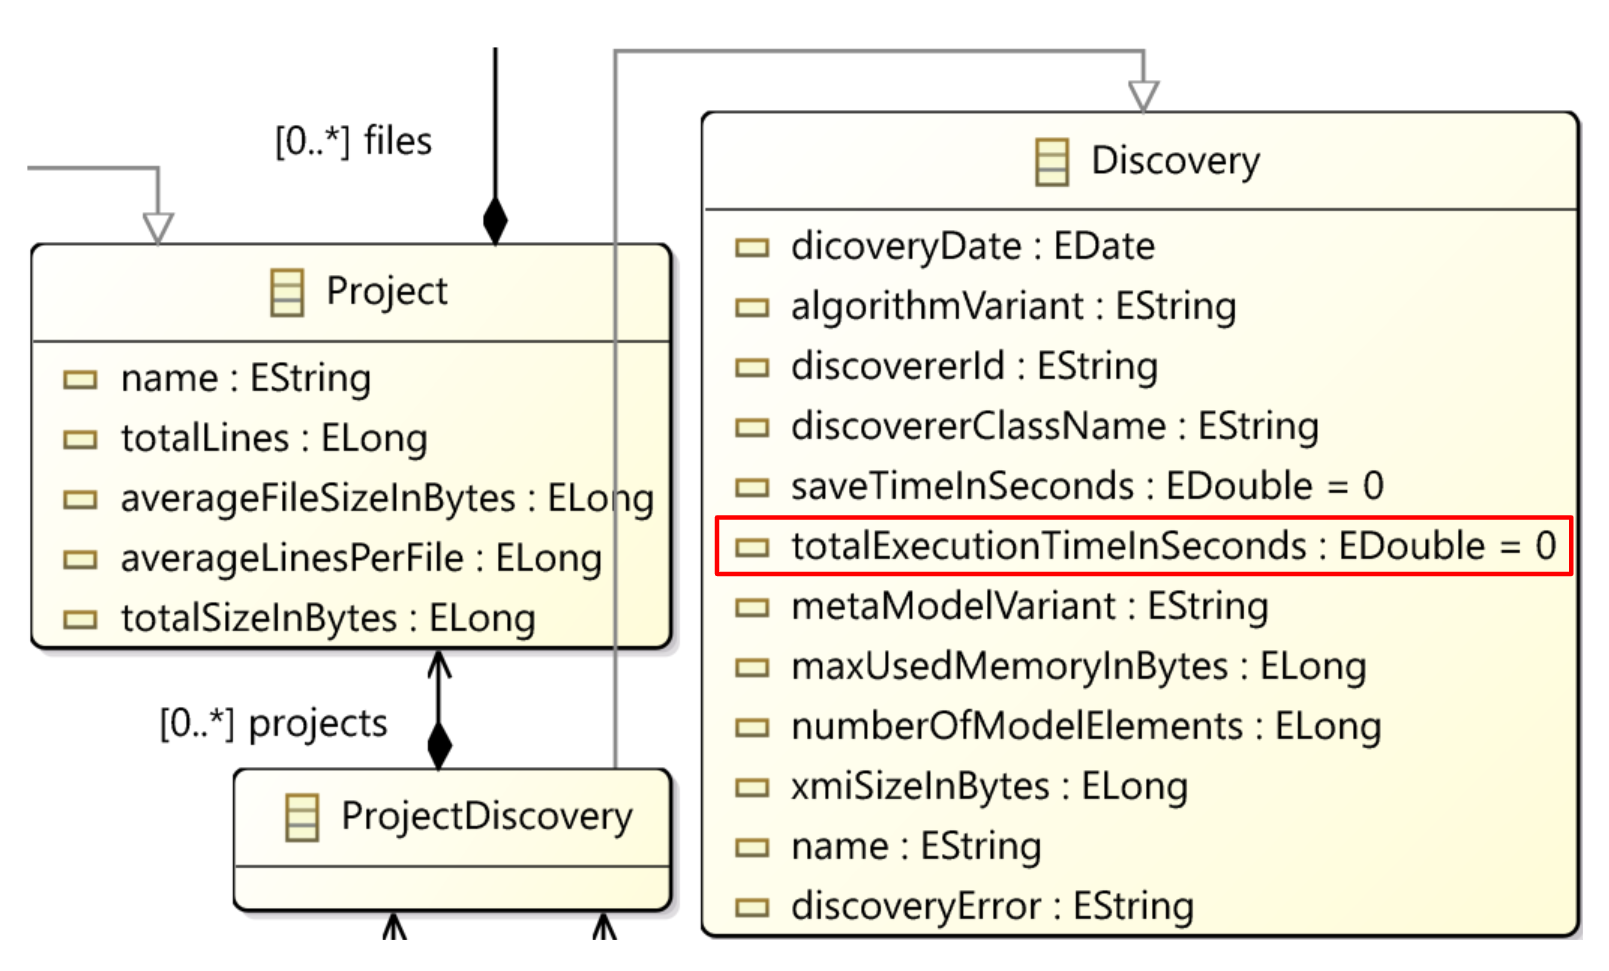
\includegraphics[width=0.7\textwidth]{./pics/chapter2pics/excerptmodisco.png}
	
	\caption{Excerpt of Modisco Benchmark metamodel in version 0.9.0.}
	\label{fig:excerptmodisco}
	%\vspace{-5mm}
\end{figure*}

\setulcolor{green} 



%\setulcolor{green} 

\begin{lstlisting}[language=Java,breaklines=true,mathescape,literate={\-}{}{0\discretionary{-}{}{}},caption=Excerpt of a directly impacted test in Modisco.\label{lis:Modisco_impactedtest_V2}]
	@Test(timeout=4000)
	public void test000() throws Throwable {
		DiscoveryIterationImpl discoveryIterationImpl0 = new DiscoveryIterationImpl();
		...
		assertFalse(discoveryIterationImpl0.eIsProxy());
		assertEquals(0.0,  (*\ul{discoveryIterationImpl0.getDiscoveryTimeInSeconds()}*), 0.01);
		assertTrue(discoveryIterationImpl0.eDeliver());
		assertEquals(0.0, discoveryIterationImpl0.getSaveTimeInSeconds(), 0.01);
		assertEquals(0L, discoveryIterationImpl0.getMaxUsedMemoryInBytes());
		assertTrue(discoveryIterationImpl0.eDeliver());
		...
	}
	
	
\end{lstlisting}

\begin{lstlisting}[language=Java,breaklines=true,mathescape,literate={\-}{}{0\discretionary{-}{}{}},caption=Excerpt of an indirectly impacted test in Modisco.\label{lis:Modisco_indirectimpactedtest_V2}]
	@Test(timeout = 4000)
	public void test16()  throws Throwable  {
		DiscoveryIterationImpl discoveryIterationImpl0 = new DiscoveryIterationImpl();
		EList<Event> eList0 = discoveryIterationImpl0.getMemoryMeasurements();
		try { 
			discoveryIterationImpl0. (*\ul{eSet(30, (Object) eList0)}*);
			fail("Expecting exception: ClassCastException");
			
		} catch(ClassCastException e) {
			verifyException("org.eclipse.modisco.infra.discovery.benchmark.impl.DiscoveryIterationImpl", e);
		}
		assertEquals(0.0, discoveryIterationImpl0.getSaveTimeInSeconds(), 0.01);
		...
	}
	
\end{lstlisting}



\begin{lstlisting}[language=Java,breaklines=true,mathescape,literate={\-}{}{0\discretionary{-}{}{}},caption=Excerpt of an impacted method in Modisco.\label{lis:Modisco_eSetmethod_V2}]
	@Override
	public void eSet(int featureID, Object newValue) {
		switch (featureID) {
			...
			case BenchmarkPackage.DISCOVERY_ITERATION__DISCOVERY_TIME_IN_SECONDS:
			(*\ul{setDiscoveryTimeInSeconds((Double)newValue)}*);
			return;
			case BenchmarkPackage.DISCOVERY_ITERATION__SAVE_TIME_IN_SECONDS:
			setSaveTimeInSeconds((Double)newValue);
			return;
			case BenchmarkPackage.DISCOVERY_ITERATION__MAX_USED_MEMORY_IN_BYTES:
			setMaxUsedMemoryInBytes((Long)newValue);
			return;
			...
		}
		
		
	\end{lstlisting}
	
\section{Approach}
\label{sec_approach}
This section presents our proposed overall approach. It first gives an overview. Then, it describes how to detect the metamodel changes and how to trace their impacts until the tests and map them. Finally, it details our prototype implementation. 




\subsection{Overview}

\red{The overall objective of our approach is to help developers in checking the behavioral correctness of the code co-evolution when metamodels evolve, as the co-evolution may be done incorrectly or in an incomplete way (i.e., referred to as partial co-evolution in \cite{le2021untangling,zaidman2011studying}). 
	Several ways exist, such as using formal methods, manual code review, or unit tests, etc. Our scope lies in tracing the impact of the metamodel changes till the tests and rely on them as an indicator for behavioral correctness of the code co-evolution, similarly as in a regression testing method \cite{leung1989insights,yoo2012regression,wong1997study}. Our vision is rather than letting the developers execute all test suite in both versions and manually analyzing them, we can reduce the set of tests to be analyzed to the only minimum necessary one. Thus, saving effort and time for developers.}  

%As depicted in 
Figure \ref{fig:appraoch} depicts the overall approach workflow. We first compute the difference between the two metamodel versions each of them having a generated code and an additional code (step {\small\boxed{1}}). In the original version, the additional code is the impacted one, and in the evolved version, the additional code is the co-evolved one. 
After that, we run the impact and the test tracing analysis to link the metamodel changes to the impacted and co-evolved code and their respective tests (step {\small\boxed{2}}). Therefore, a developer can run the traced tests before and after the code co-evolution to check their behavioral correctness. Finally, to ease this task, we map the traced tests and execute them to report them back in a form of a diagnostic to the developers for an easier in-depth analysis of the effect of metamodel evolution rather than analyzing the whole test suite (step {\small\boxed{3}}). 
\blue{Therefore, in a nutshell, there are no particular preconditions to our approach except having available code and tests from both before and after co-evolution along with the delta of the metamodel changes.} 


\begin{figure*}[tb]
	\centering
	% \hspace*{-2em}
	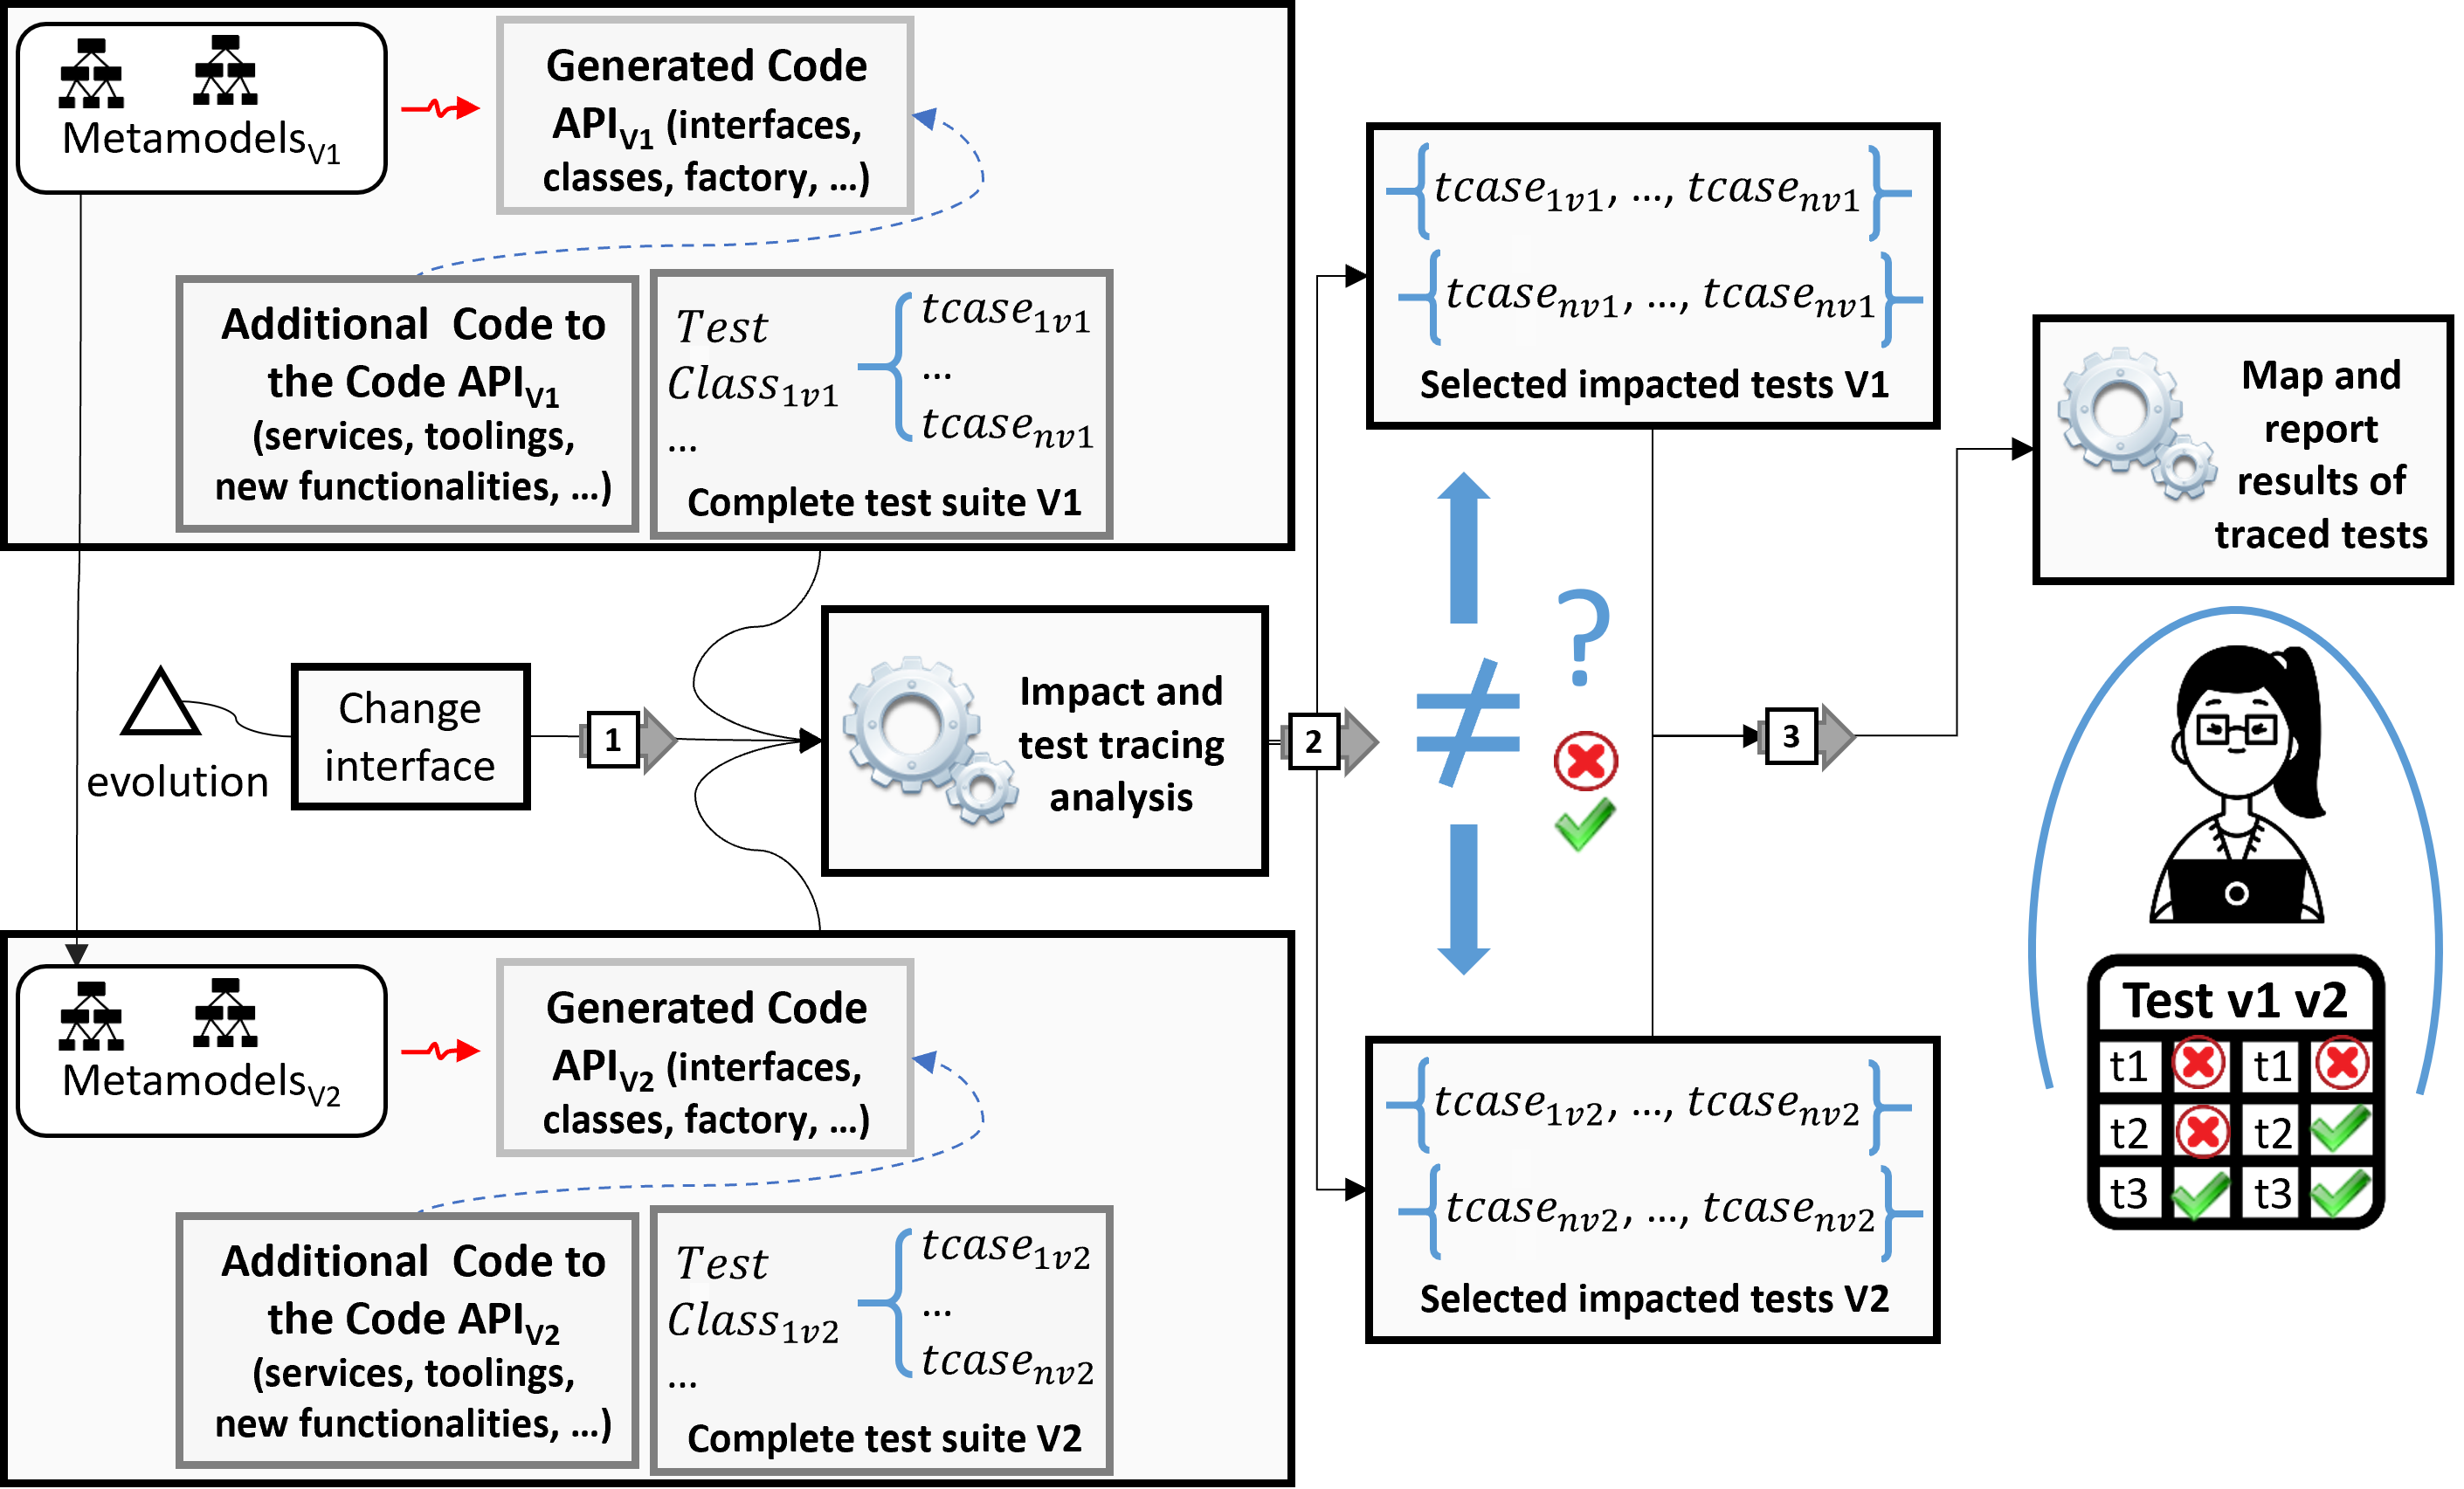
\includegraphics[width=1\textwidth]{./pics/chapter2pics/OverallApproachV2.png}
	\caption{Overall approach}
	\label{fig:appraoch}
	%\vspace{-5mm}
\end{figure*}


\subsection{Detection of metamodel Changes}\label{sec:changes}


%Software artifacts continuously evolve over time~\cite{mens2008introduction}.
%As any artifact, metamodels evolve as well.  
%Two types of changes are known and considered in the literature for metamodel evolution: \emph{atomic} and \emph{complex} changes \cite{Herrmannsdoerfer2011}. 
%Atomic changes are additions, removals, and updates of a metamodel element. Complex changes consist of a sequence of atomic changes combined together~\cite{vermolen_reconstructing_2012,khelladi2015detecting}. For example, move property is a complex change where a property is moved from a source class to a target class. This is composed of two atomic changes: delete a property and add a property \cite{Herrmannsdoerfer2011}. 
%Several existing approaches allow to automatically detect metamodel changes between two versions, such as \cite{Alter2015, williams2012searching,cicchetti_managing_2009,langer_posteriori_2013,vermolen_reconstructing_2012,Khelladi2016}.

As described in Chapter \ref{mmchanges}, we use an interface specification of changes {\small\boxed{1}} that is a connection layer to our test tracing approach with the existing change detection approaches~\cite{Alter2015, williams2012searching,cicchetti_managing_2009,langer_posteriori_2013,vermolen_reconstructing_2012,Khelladi2016}.

\begin{table*}[t]
	\caption{List of metamodel changes and how they are traced up to the tests in the original and evolved versions. }
	\label{tab:changes}
	\centering
	\resizebox{14.5cm}{!} {
		\hspace*{-3em}
		\begin{tabular}{lcc}
			\toprule
			& \multicolumn{2}{c}{Tests treatment} \\ \cmidrule{2-3}
			\multicolumn{1}{c}{\multirow{-2}{*}{Metamodel changes}} & In original version (V1)            & In evolved version (V2)            \\ \midrule
			$\diamond$ Delete property \emph{p} in class \texttt{C}       &   Search for usages of \emph{p} in \texttt{C}                &        \emph{n/a}          \\ \midrule
			$\diamond$ Delete class \texttt{C}          &   Search for usages of \texttt{C}               &      \emph{n/a}            \\ \midrule
			
			$\diamond$ Add property \emph{p} in class \texttt{C}     &        \emph{n/a}  & Search for  usages of\emph{p} in \texttt{C}         \\ \midrule
			$\diamond$ Add class \texttt{C}     &      \emph{n/a}       &   Search for usages of \texttt{C}                         \\ \midrule
			
			
			$\diamond$ Rename element \emph{e} to \emph{e'} in class \texttt{C}	           &  Search for usages of \emph{e} in \texttt{C}    & Search for usages of \emph{e'} in \texttt{C}                \\ \midrule
			
			\begin{tabular}[c]{@{}l@{}}$\diamond$ Change multiplicity of property \\ \emph{p} in class \texttt{C} \end{tabular}           &        \multicolumn{2}{c}{Search for usages of \emph{p} in \texttt{C}}           \\ \midrule
			
			\begin{tabular}[c]{@{}l@{}}$\diamond$ Change type of property \emph{p}  \\from \texttt{S} to \texttt{T}\end{tabular}           &      \multicolumn{2}{c}{Search for usages of \emph{p} in \texttt{C}}     \\ \midrule
			
			\begin{tabular}[c]{@{}l@{}}$\diamond$ Move property $p_{i}$ from \\ class \texttt{S} to \texttt{T} through \emph{ref}\\
				%$\diamond$ Extract class \texttt{S} to \texttt{T} \\with properties $p_{1},...,p_{n}$ \\ \red{through \emph{ref}}\\
				$\diamond$ Extract class of properties $p_{1},$\\$...,p_{n}$ from \texttt{S} to \texttt{T} through \emph{ref}\end{tabular}           &     Search for usages of all $p_{i}$ in \texttt{S}             &      Search for usages of all $p_{i}$ in \texttt{T}             \\ \midrule
			
			\begin{tabular}[c]{@{}l@{}}$\diamond$ Push property $p_{i}$ from \\class \texttt{Sup} to \texttt{Sub$_{1}$},...,\texttt{Sub$_{n}$}\end{tabular}           &    Search for usages of all $p_{i}$ in \texttt{Sup}              &    Search for usages of all $p_{i}$ in all \texttt{Sub$_{i}$}               \\ \midrule
			
			\begin{tabular}[c]{@{}l@{}}$\diamond$ Pull property $p_{i}$ from \\classes \texttt{Sub$_{1}$},...,\texttt{Sub$_{n}$} to \texttt{Sup}  \end{tabular}           &     Search for usages of all $p_{i}$ in all \texttt{Sub$_{i}$}             &    Search for usages of all $p_{i}$ in \texttt{Sup}                 \\ \midrule
			
			\begin{tabular}[c]{@{}l@{}}$\diamond$ Inline class \texttt{S} to \texttt{T} \\with properties $p_{1},...,p_{n}$\end{tabular}           &      Search for usages of all $p_{i}$ in \texttt{S}               &      Search for usages of all $p_{i}$ in \texttt{T}          \\ %\midrule
			
			%&                  &                  \\ 
			
			\bottomrule                 
		\end{tabular}
	}
\end{table*}


\blue{}In practice, we focus on the impacting metamodel changes that will require co-evolution of the code and not on the non-impacting changes. For example, a delete change or a change of type will impact the code and possibly its behavior that can be observed with its tests. 
However, addition changes, although \red{non-breaking}, can be traced back to their newly added tests. Thus, we also consider them to observe their behavior.
The list of metamodel changes \cite{iovino2012impact,cicchetti_managing_2009} we consider for tracing their impact up to the tests is as shown in the first column of Table \ref{tab:changes}. 

For each version of the tests, we use different information provided by each metamodel change, depending on whether we are tracing the impacted tests in the original or the evolved versions. Columns 2 and 3 of table \ref{tab:changes} detail the treatments of each metamodel change in the original and evolved versions. For example, for a rename element \emph{e} to \emph{e'}, we search for \emph{e} and \emph{e'}, respectively, in the original and evolved versions. Similarly, for the other changes, such as Move, Pull, Push, etc. where the source and target classes are different in the original and evolved versions. Only the impact of delete changes is searched in the original version, while the impact of addition changes is only searched in the evolved version. 





\subsection{Tracing the Impacted Tests}
\label{section: tracing the impacted tests}
\red{}


Our approach traces the impact of metamodel changes up to the test. To do that, we structure the code source to better navigate in it. 
Before starting, we parse the code source including tests and build the Code Call Graph (CCG) at the methods level. It consists of nodes $\mathbb{N}$ that are methods, and edges $\mathbb{E}$ that are calls between methods. 
For a given method, the CCG allows us to retrieve its callers, hence, tracing the call methods recursively up to the tests. %map between the code elements (CE) and their usages in the code (CEU). After that, we link the %, as shown in Table \ref{x}.
After that, we apply Algorithm \ref{algo :impactedTestsDetection} on the built CCG. Overall, for each detected metamodel change, the algorithm computes the list of direct and indirect impacted tests that can be traced to the given metamodel change. 


First, we analyze the AST of the code to identify the code usages of the evolved metamodel element. The information concerning the metamodel element before and after evolution, which is included in the metamodel change (see Table \ref{tab:changes}), allow us to spot the impacted code usages (Line 1). For example, for a rename property \emph{id}, the algorithm will first find its usages, such as \emph{getId()} or \emph{setId()}\footnote{\blue{Note that the knowledge about the generated code elements from the metamodel elements (e.g., getter/setter for EAttribute, class/interface for EClass, etc.) is so far hard-coded in the implementation of Algorithm \ref{algo :impactedTestsDetection}. The mappings must be provided for our approach to be able to trace the tests.}}. 
%
Then, we filter these impacted code usages by keeping only the ones found inside a method declaration. % for example : variable declaration or an If condition clause, etc. 
Let us call the found method declaration using the impacted code \textit{IM()} (Line 5). If \textit{IM()} is a test method, that means that we found a direct impacted test (Line 7). Otherwise, thanks to the CCG, we retrieve \textit{IM()}'s parents \emph{parentsOfIM}, which are all the method declarations invoking IM() (Line 9-17). 
%
Afterwards and recursively, we check each parent of \textit{IM()} if it is a test method or not (Line~14). The process is finished if we reach a method declaration that has no parents in the CCG that is either a test or not, or if the reached method declaration is already treated in the \emph{parentsOfIM}. Therefore, by design, after browsing all the impacted code usages, Algorithm \ref{algo :impactedTestsDetection} traces the list of all impacted tests, without missing any if impacted. \red{It is worth noting that tracing all impacted tests holds syntactically and w.r.t. static semantics. Possible side-effect will require further advanced dynamic analysis and is left for future work.} 
Listing \ref{lis:Modisco_impactedtest_V2} presents an example of an impacted test in the Eclipse Modisco.infra.discovery.benchmark project. 
\red{As described in Section \ref{sec:changes}, we detect that the attribute setTotalExecutionTimeInSeconds is renamed and moved from the class Discovery to the class DiscoveryIteration. After that, Algorithm \ref{algo :impactedTestsDetection} detects the code usage \emph{getDiscoveryTimeInSeconds}. Then, it traces it to the method \emph{test000}. As it has the \emph{@Test} annotation, we conclude that \emph{test000} is an impacted test due to the detected move change. 
	%
	Note that a test can be impacted by multiple metamodel changes, and one metamodel change can impact many tests. Algorithm \ref{algo :impactedTestsDetection} will detect either cases. 
}

\setulcolor{green} 


\subsection{Mapping of impacted tests}

%this would allow to build a summary table between v1 v2 of the mapped table
After having traced the impacted tests, we further assist developers in analyzing the output of our approach. We provide a diagnostic in a form of a visualized report. This report displays the mapping of impacted tests between the original and evolved versions, along with the verdict of their execution (i.e., pass, fail, and error) and the corresponding impacted change. As an input to generate the diagnostic, the developer selects two impacted traced test classes in the original and evolved versions.
%select two test classes that represent the same impacted test class from the first and second versions. 
The mapping between the two sets of test cases for these classes is performed using a state-of-the-art tool, namely GumTree \cite{falleri2014fine}. It parses both test classes into a tree structure to enable the matching of the test cases. Herein, we distinguish three cases, namely:~1) tests that exist in both versions,~2) tests that exist in the original version but not in the evolved one, and~3) tests that exist in the evolved version but not in the original one.
The impacted tests are then executed programmatically using JUnit runner. To facilitate the analysis and the tracing of impacted tests, we include the corresponding impacting metamodel changes in an additional column of the diagnostic report.  

\definecolor{circlegreen}{HTML}{7ed321}
\begin{algorithm}
	\caption{Impacted tests detection}\label{algo :impactedTestsDetection}
	\begin{algorithmic}[1]
		%\textbf{Input :}{codeCallGraph, change}
		
		
		\Require codeCallGraph, change
		%\Ensure $y = x^n$ 
		\State impactedUsages $\leftarrow$ match(AST, change)
		
		\State impactedTests $\leftarrow \phi$ 
		\For {(impactedUsage $\in$ impactedUsages )}
		
		\State \emph{\textcolor{circlegreen}{ \footnotesize{/* Find the method declaration using impactedUsage*/}}}
		
		\State IM $\leftarrow$ getIM(impactedUsage, codeCallGraph) 	       
		\If{(isTest(IM))}
		
		\State   impactedTests.add(IM) 	\emph{\textcolor{circlegreen}{/*If not already added*/}}
		
		\Else
		
		\State parentsOfIM $\leftarrow$ getParents(IM, codeCallGraph)
		
		\State  nextRound.add(parentsOfIM)
		
		\While{(nextRound.hasNewIMs())}
		
		\State    IM $\leftarrow$ nextRound.get()
		
		
		\If{(isTest(IM)}
		
		\State  impactedTests.add(IM)\emph{\textcolor{circlegreen}{/*If not already added*/}}
		
		\Else 
		
		\State  parentsOfIM $\leftarrow$ getParents(IM, codeCallGraph)
		
		\State   nextRound.add(parentsOfIM) 
	%	\EndIf
		
		
		
		
%		\EndWhile
	%	\EndIf
	%	\EndFor
	\end{algorithmic}
\end{algorithm}


\red{Figure \ref{fig:toolView} illustrates a screenshot of the test tracer report on a toy example "Employee Management Project". After selecting the class of tests that have been traced before code co-evolution, and the class of tests that have been traced after code co-evolution, the user clicks on "Map tests" to display the table of mapped tests with their verdict of execution.
	To illustrate the verdict of the test execution, we made: the passing test in \textcolor{green}{green}, the failing test in \textcolor{blue}{blue}, and erroneous tests in \textcolor{red}{red}. For example, the change "Delete Class Contact" impacts two tests, test11 which passes, and test06 which fails. The verdict of the execution of the tests has no relation with the change itself but with the test that uses the code elements impacted by the metamodel change. Those tests do not exist anymore in the evolved version since the class Contact is absent and cannot be tested anymore.}




\subsection{Tool implementation}

We implemented our solution as an Eclipse Java plugin handling Ecore/EMF metamodels and their Java code. %a state-of-the-art
We rely on our approach \cite{khelladi2015detecting} to perform the detection of the metamodel changes bridged with the change interface. 
The test tracing, technically, consists of parsing the java code and manipulating its AST using JDT eclipse plugin\footnote{Eclipse Java development tools (JDT): \url{https://www.eclipse.org/jdt/core/}} to construct the Code Call Graph (CCG). After that, we navigate within the methods calls until we either reach a test or not. Finally, for each impacted \emph{TestClass}, we create a copy \emph{TestClass\_Impacted} where we only include the impacted traced test cases. The developer can then launch the traced tests in both the original and evolved versions to investigate the behavioral correctness of the co-evolved code. 
%The tests' AST nodes are manipulated with edit actions %: modified, replaced or removed)  
%using the package \textit{ org.eclipse.jdt.core.dom.rewrite} and \textit{org.eclipse.core.filebuffers}. 
%\red{say more or reformulate above}
%
We further implemented the diagnostic report as a view that shows the mapped tests with GumTree~\cite{falleri2014fine}, their verdict retrieved programmatically using JUnit Runner\footnote{\url{https://junit.org/junit4/javadoc/4.13/org/junit/runner/Runner.html}} and impacting metamodel changes, as shown in Figure~\ref{fig:toolView}. The goal is to ease the developers' in-depth analysis of the effect of metamodel evolutions rather than rerunning and analyzing the whole test suite.

\begin{figure*}[tb]
	\centering
	%\hspace*{-1em}
	% \vspace{-5mm}
	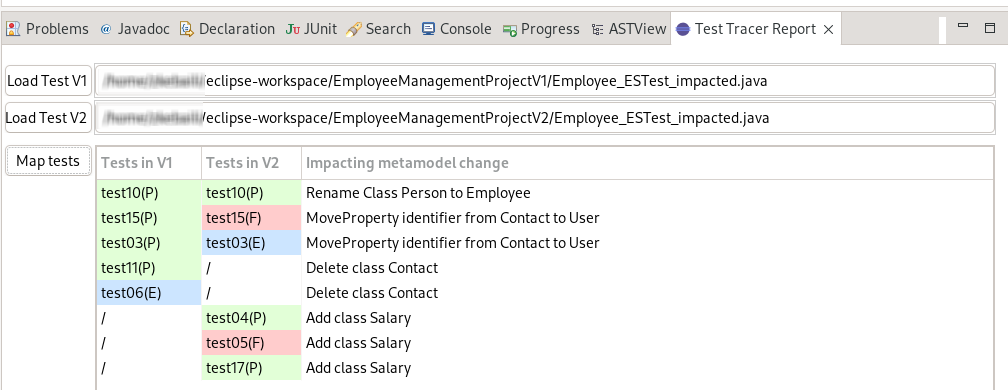
\includegraphics[width=1\textwidth]{./pics/chapter2pics/TestTraceReport.png}
	%\caption{Artifacts and structure of a software language in the Eclipse platform.}
	\caption{A snippet of the diagnostic report view to visualize and analyze the traced impacted tests.}
	\label{fig:toolView}
	%\vspace{-5mm}
\end{figure*}
\section{Evaluation}
\label{sec_evaluation}
This section evaluates our automatic approach of checking the behavioral correctness of the metamodel and code co-evolution. 
First, we present the data set and the evaluation process. Then, we set the research questions we address and discuss the obtained results.


\begin{table*}[t]
	\centering
	
	\caption{Details of the metamodels and their evolutions.}
	\label{CaseStudies_Evolution}
%	\hspace*{-1em}
	\resizebox{16cm}{!} {
		\hspace*{-2em}
		\begin{tabular}{llll}
			\toprule
			\begin{tabular}[c]{@{}l@{}}Evolved metamodels\end{tabular}                 & Versions & %\begin{tabular}[c]{@{}l@{}}Size ($N^{o}$ of\\ elements)\end{tabular} &
			\multicolumn{1}{c}{\begin{tabular}[c]{@{}c@{}}Atomic changes \\in the metamodel\end{tabular}} & \multicolumn{1}{c}{\begin{tabular}[c]{@{}c@{}}Complex changes \\in the metamodel\end{tabular}} \\ \midrule		
			
			%\multirow{6}{*}{\begin{tabular}[c]{@{}l@{}}OCL\end{tabular}} 
			\begin{tabular}[c]{@{}l@{}}Pivot.ecore \\ in project\\\emph{ocl.examples.pivot}\end{tabular}                        &  \begin{tabular}[c]{@{}l@{}}3.2.2 \\ to\\ 3.4.4\end{tabular}        &   %\begin{tabular}[c]{@{}l@{}}Original: 1473 \\Evolved: 1787\end{tabular}  &
			\begin{tabular}[c]{@{}l@{}} \emph{Deletes:} 2 classes, 16 properties, 6 super types \\ \emph{Renames:} 1 class, 5 properties \\ \emph{Property changes:} 4 types;  2 multiplicities \\ \emph{Adds:} 25 classes, 121 properties,  36 super types  \end{tabular}                                                         &    \begin{tabular}[c]{@{}l@{}} 1 pull property \\ 2 push properties  \end{tabular}                                                        \\ \midrule %cmidrule{2-5} %midrule	
			
			\begin{tabular}[c]{@{}l@{}}Pivot.ecore \\ in project\\\emph{ocl.pivot}\end{tabular}                        &  \begin{tabular}[c]{@{}l@{}}6.1.0 \\to\\ 6.7.0 \end{tabular}        &    \begin{tabular}[c]{@{}l@{}} \emph{Deletes:} 0 classes, 4 properties, 4 super types \\ \emph{Renames:} 0 class, 1 properties \\ \emph{Property changes:} 49 types;  \\ \emph{Adds:} 5 classes, 47 properties,  7 super types  \end{tabular}    &   n/a \\ \midrule
			
			%\begin{tabular}[c]{@{}l@{}}Pivot.ecore in \\ project\\ocl.pivot\end{tabular}                        &  \begin{tabular}[c]{@{}l@{}}6.7.0 \\to\\ 6.18.0 \end{tabular}        &    \begin{tabular}[c]{@{}l@{}} \emph{Deletes:} 0 classes, 0 properties, \\ 0 super types \\ \emph{Renames:} 0 class, 1 properties \\ \emph{Property changes:} 5 types; \\  0 multiplicities \\ \emph{Adds:} 1 classes, 4 properties, \\ 1 super types  \end{tabular} & n/a   \\ 
			
			\begin{tabular}[c]{@{}l@{}}ExtendedTypes.ecore \\in project\\\emph{papyrus.infra.extendedtypes}\end{tabular}            & \begin{tabular}[c]{@{}l@{}}0.9.0 to\\ 1.1.0\end{tabular}         & %\begin{tabular}[c]{@{}l@{}}Original: 40 \\Evolved: 57\end{tabular}     &   
			\begin{tabular}[c]{@{}l@{}}Deletes: 10 properties, 2 super types \\ Renames: 3 classes, 2 properties \\ Adds: 8 classes, 9 properties, 8 super types  \end{tabular}                                                      &    \begin{tabular}[c]{@{}l@{}} 2 pull property \\ 1 push property \\ 1 extract super class \end{tabular} \\ \midrule
			
			\begin{tabular}[c]{@{}l@{}}Benchmark.ecore \\ in project \\ \emph{modisco.infra.discovery.benchmark}\end{tabular}                & \begin{tabular}[c]{@{}l@{}}0.9.0 to\\ 0.13.0\end{tabular}         &   %\begin{tabular}[c]{@{}l@{}}Original: 95 \\Evolved: 106\end{tabular}    &  
			\begin{tabular}[c]{@{}l@{}} Deletes: 6 classes, 19 properties, 5 super types \\ Renames: 5 properties  \\ Adds: 7 classes, 24 properties, 4 super types  \end{tabular}                                                        &     \begin{tabular}[c]{@{}l@{}} 4 moves property \\ 6 pull property \\ 1 extract class \\ 1 extract super class \end{tabular}    
			\\ \midrule
			\midrule
			
			\begin{tabular}[c]{@{}l@{}}Ecore.ecore \\ in project \\ \emph{org.eclipse.emf}\end{tabular}                & \begin{tabular}[c]{@{}l@{}}2.37.0 to\\ 2.37.0'\end{tabular}         &   %\begin{tabular}[c]{@{}l@{}}Original: 95 \\Evolved: 106\end{tabular}    &  
			\begin{tabular}[c]{@{}l@{}} Deletes: 1 class, 2 properties \\ Renames: 2 properties  \\   \end{tabular}                                                        &     \begin{tabular}[c]{@{}l@{}} 1 move property \\ 1 pull property  \end{tabular}    
			\\ 
			
			\bottomrule                                         
		\end{tabular}
	}
	%\vspace{-1em}
\end{table*}


\subsection{Data Set}

This section presents the used data set in our evaluation to be found in the attached supplementary material\footnote{\url{https://figshare.com/s/b6251b9e47fa82983ce5}}. 



We evaluate our approach on four case studies of language implementations in Eclipse, namely OCL \cite{MDTOCL}, Modisco \cite{MDTModisco}, Papyrus \cite{MDTPapyrus}, and EMF \cite{EclipseEMF} project. 
%
OCL is a standard language defined by the Object Management Group (OMG) to specify First-order logic constraints. Modisco is an academic initiative to support development of model-driven tools, reverse engineering, verification, and transformation of existing software systems. 
Papyrus is an industrial project led by CEA\footnote{\url{http://www-list.cea.fr/en/}} to support model-based simulation, formal testing, safety analysis, etc. 
\red{The EMF project is a modeling framework and code generation facility for building tools and other applications based on a structured data model \cite{steinberg2008emf}.}  
Thus, the four case studies cover standard, academic, and industrial languages that have evolved several times for more than 10 years of continuous development period. 

Moreover, we aimed at selecting meaningful evolutions that do not consist in only deleting metamodel elements, but rather include complex evolution changes. We also aimed to select long and short evolution intervals in the selected releases versions to stress test our approach in different scenarios. 
\red{This is the case for the OCL, Modisco, and Papyrus case studies. However, they do not have manually written tests. Thus, we added the EMF case study that have manually written tests, but its metamodel is stable with no evolutions. Therefore, we had to simulate a set of metamodel evolution changes similar to those real-world changes observed in our three first case studies and we co-evolved their impacts with our previous work  \cite{Khelladi2020}.} 


Table \ref{CaseStudies_Evolution} gives details about the selected case studies, in particular about their metamodels and the changes applied during evolution. 
%\red{Also about the code and tests details in each project.}
The total of applied metamodel changes was \red{452} atomic changes and \red{21} complex changes in the five metamodels.
%
Table~\ref{CaseStudies_CoEvolution} gives details on the size of the projects in terms of code and tests of the original and evolved versions. 
We collected a total of~18 projects to evaluate our approach on.  



\subsection{Evaluation Process}

\red{We evaluate our approach by: 1) investigating its usefulness compared to the manual tracing of the impacted tests with user study, 2) measuring its ability to automatically trace the impacted tests due to impacting metamodel changes both in the original and evolved version of the project, 3) assessing its ability to give an indication about the correctness of the code and metamodel co-evolution, and finally 4) measuring the gains of its usage in terms of reduction of tests and their execution time.} Note that as the metamodel changes are taken as input of our automatic test tracing, we studied the original and evolved versions to confirm the metamodel changes. Therefore, we do not take an incorrect input of metamodel changes that would mislead our traced tests, which would mislead the behavioral checking of the code co-evolution. 


\red{Regarding the tests, only the EMF case study had manually written tests. Thus, we had to generate tests for OCL, Modisco, and Papyrus case studies. We used 
	a state-of-the-art tool, namely EvoSuite~\cite{fraser2011evosuite}. 
	EvoSuite is a search-based tool for Unit Tests generation. It uses a heuristic algorithm, particularly, genetic algorithm
	% ( explain different elements of it ?)
	in the Test Suit generation. In their used approach Fraser et al.~\cite{fraser2011evosuite} aimed to maximize the coverage metric and mutation score which guarantees good-quality tests. 
	EvoSuite is largely used and it was evaluated not only in literature but also in the industrial context. Firhard et al.~\cite{10.1007/978-3-031-21251-2_2} compared it with DSpot, a state-of-the-art tool for test amplification, their results show that EvoSuite achieves a statistically better mutation score. Herculano et al. found that EvoSuite's generated tests can successfully help to identify faults during maintenance tasks~\cite{9954000}. In industry, Rozière et al. use automated tests generated with EvoSuite to filter invalid code translations in the context of their work done for Meta \cite{roziere2021leveraging}. 
	Gruber et al.~\cite{gruber2023automatic} further showed the quality and robustness of the generated tests. It showed that while flakiness is at least as common in generated tests as in developer-written tests, EvoSuite is effective in alleviating this issue giving~71.7\% fewer flaky tests. Thus, EvoSuite is appropriate in our work to generate robust tests in the original code and in the co-evolved code to compare their results, i.e., check behavioral correctness.} 
We simply let EvoSuite run to generate Junit test classes for the selected projects with the following parameters: \emph{-DmemoryInMB=2000 -Dcores=4 -DtimeInMinutesPerClass=10 evosuite:generate evosuite:export}. It uses up to 2GO of RAM, 4 CPU cores, and 10 minutes per test class. 
Generating tests is a best practice, in particular w.r.t. its efficiency in test generation and at a large scale for all public methods \cite{DANGLOT2019110398,https://doi.org/10.1002/stvr.1601}. 
EvoSuite generates tests for all public methods, whereas developers tend to manually write a few tests for only some targeted methods. Thus, relying only on manually written tests increases the risk of not assessing the behavioral correctness of many cases of code co-evolutions that are not covered by test cases. Generating tests alleviates this risk. 
\red{Indeed, this is observed when computing the coverage metric for each of our considered projects. Table \ref{table:coverage} shows that the highest coverage (69\% to 95\%) is obtained on projects with automatically generated tests and the lowest coverage (17\% to 33\%) were on the two projects with manually written tests.}  






\begin{table*}[t]
	\centering
	\caption{Details of the projects and their tests.}
	\label{CaseStudies_CoEvolution}
	\hspace*{-2em}
	\resizebox{14.5cm}{!} {
		\begin{tabular}{lcccccc}
			\toprule
			\begin{tabular}[c]{@{}l@{}}Projects co-evolved in response to the evolved \\ metamodels \end{tabular} 	& \begin{tabular}[c]{@{}c@{}}$N^{o}$ of \\ packages\end{tabular} & \begin{tabular}[c]{@{}c@{}}$N^{o}$ of \\ classes\end{tabular} & %\begin{tabular}[c]{@{}c@{}}N° of \\ methods\end{tabular} & 
			\begin{tabular}[c]{@{}c@{}}$N^{o}$ of test\\ packages\end{tabular} & \begin{tabular}[c]{@{}c@{}}$N^{o}$ of test\\ classes\end{tabular} &
			\begin{tabular}[c]{@{}c@{}}$N^{o}$ of \\ LOC\end{tabular} & \begin{tabular}[c]{@{}c@{}}$N^{o}$ of \\ tests\end{tabular} %& \begin{tabular}[c]{@{}c@{}}$N^{o}$ of total \\ direct errors \end{tabular}& \begin{tabular}[c]{@{}c@{}}$N^{o}$ of total \\ indirect errors \end{tabular}
			\\ \midrule		
			
			$[P1_{V1}]$ ocl.examples.pivot & 22 & 439 &22  & 290 & 74002 & 7322 \\ \midrule
			
			$[P1_{V2}]$ ocl.examples.pivot & 22 & 480 & 22 &220 &  89449& 4990 \\ \midrule
			
			$[P2_{V1}]$ ocl.examples.base & 12 & 181 & 12 &119 &17617 & 2320 \\ \midrule
			
			$[P2_{V2}]$ ocl.examples.base & 12 & 181 & 12 & 118&17596 & 2133 \\ \midrule
			
			
			$[P3_{V1}]$ ocl.pivot & 60 & 1006 & 55 &598 & 142236& 8795 \\ \midrule
			
			$[P3_{V2}]$ ocl.pivot & 63 & 1090 & 58 & 683&153613 & 6396 \\ \midrule
			
			%$[P3_{V3}]$ ocl.pivot & 66 & 1143 & 61 & 738&164845 & 6356 \\ \midrule
			
			$[P4_{V1}]$ papyrus.infra.extendedtypes & 7 & 37 &7  & 19 & 2057 & 135 \\ \midrule
			
			$[P4_{V2}]$ papyrus.infra.extendedtypes & 7 & 51 & 7 &26 &  2570 & 248 \\\midrule
			$[P5_{V1}]$ papyrus.infra.extendedtypes.emf & 5 & 25 &4  & 14 & 1145 & 104 \\ \midrule
			
			$[P5_{V2}]$ papyrus.infra.extendedtypes.emf & 5 & 25 & 4 &14 &  1145& 104 \\ \midrule
			$[P6_{V1}]$ papyrus.uml.tools.extendedtypes & 5 & 15 &3  & 9 & 726 & 75 \\ \midrule
			
			$[P6_{V2}]$ papyrus.uml.tools.extendedtypes & 5 & 15 & 3 &9 &  725& 75 \\ \midrule
			
			$[P7_{V1}]$ org.eclipse.modisco.infra.discovery.benchmark & 3 &  28& 3 &15 & 2333 &524  \\ \midrule
			
			$[P7_{V2}]$ org.eclipse.modisco.infra.discovery.benchmark &3  & 30 &3  & 15&  2588& 619 \\%\midrule
			
			
			% \begin{tabular}[c]{@{}l@{}}$[P1]$ ocl.examples.pivot\\ $[P2]$ ocl.pivot\end{tabular}      &   \begin{tabular}[c]{@{}l@{}}22\\// \end{tabular}     & \begin{tabular}[c]{@{}l@{}}439\\?? \end{tabular}                 &                                          %  \begin{tabular}[c]{@{}l@{}}5445\\1984 \end{tabular}              & 
			%\begin{tabular}[c]{@{}l@{}}74002\\// \end{tabular} & \begin{tabular}[c]{@{}l@{}} ??\\?? \end{tabular} %& \begin{tabular}[c]{@{}l@{}} 489\\27 \end{tabular} & \begin{tabular}[c]{@{}l@{}} 37\\2 \end{tabular} 
			%\\ \midrule	
			
			% \begin{tabular}[c]{@{}l@{}}$[P1]$ ocl.examples.pivot\\ $[P2]$ ocl.pivot\end{tabular}      &   \begin{tabular}[c]{@{}l@{}}22\\// \end{tabular}     & \begin{tabular}[c]{@{}l@{}}439\\?? \end{tabular}                 &                                          %  \begin{tabular}[c]{@{}l@{}}5445\\1984 \end{tabular}              & 
			%\begin{tabular}[c]{@{}l@{}}74002\\// \end{tabular} & \begin{tabular}[c]{@{}l@{}} ??\\?? \end{tabular} %& \begin{tabular}[c]{@{}l@{}} 489\\27 \end{tabular} & \begin{tabular}[c]{@{}l@{}} 37\\2 \end{tabular} 
			%\\ %\midrule	
			\midrule		
			\midrule
			$[P_{ecore\_V1}]$ org.eclipse.emf.ecore & 13 & 168& /& / & 142586 & 0 \\
			\midrule
			$[P_{ecore\_V2}]$ org.eclipse.emf.ecore & 13 & 166 & /  & / & 141434 & 0 \\ 
			
			\midrule
			
			
			$[P8_{V1}]$ org.eclipse.emf.test.core & / & / &19 & 141 & 40858 & 322 \\
			\midrule
			$[P8_{V2}]$ org.eclipse.emf.test.core & / & / &19  & 141 & 40544 & 322 \\ 
			
			\midrule
			
			$[P9_{V1}]$ org.eclipse.emf.test.xml & / & / & 6& 27 & 12088 & 64 \\
			\midrule
			$[P9_{V2}]$ org.eclipse.emf.test.xml & /& / &6  & 27 & 12088 & 64 \\ 
			
			
			\bottomrule		
		\end{tabular}
	}
	
\end{table*}

\begin{table*}[t]
	%\begin{wraptable*}{r}{5.5cm}
	\centering
	\caption{Coverage metric of each evaluation project.} 
	\label{table:coverage}
	%
	%\small
	%\hspace*{-2em}
	\resizebox{11cm}{!}{
		\begin{tabular}{
				@{\hskip3pt}c@{\hskip3pt}|c@{\hskip3pt}|c@{\hskip3pt}|c@{\hskip3pt}|c@{\hskip3pt}|c@{\hskip3pt}|c@{\hskip3pt}|c@{\hskip3pt}|| c@{\hskip3pt} |c@{\hskip3pt} }
			\toprule 
			Projects
			& \begin{tabular}[c]{@{}l@{}}$[P1]$ \end{tabular}
			& \begin{tabular}[c]{@{}l@{}}$[P2]$ \end{tabular} &\begin{tabular}[c]{@{}l@{}} $[P3]$  \end{tabular}
			&\begin{tabular}[c]{@{}l@{}} $[P4]$\end{tabular}
			&\begin{tabular}[c]{@{}l@{}} $[P5]$\end{tabular}
			& \begin{tabular}[c]{@{}l@{}}$[P6]$ \end{tabular} 
			& \begin{tabular}[c]{@{}l@{}}$[P7]$ \end{tabular}
			&\begin{tabular}[c]{@{}l@{}}$[P8]$ \end{tabular}
			&\begin{tabular}[c]{@{}l@{}}$[P9]$ \end{tabular}\\ \midrule%{2-10}
			
			
			\begin{tabular}[c]{@{}l@{}}Coverage V1 \end{tabular} &  66.9\%  &  86.1\%    &   80.1\%  &  95.6\%  &   95.1\%    &   89.5\%   &   91.3\% &  18\%  &  33.4\%   \\ 
			\midrule%{2-10}
			
			
			\begin{tabular}[c]{@{}l@{}}Coverage V2 \end{tabular} &  66.2\%  &  85.4\%    &   74.1\%  &  95.2\%  &   95.2\%    &   89.2\%   &   87.5\% &   17.2\% &  33\%    \\ 
			
			
			\bottomrule
		\end{tabular}
	}
	%\end{wraptable*} 
	%\vspace{-1em}
\end{table*}

\subsection{Research Questions}
This section sets the research questions (RQs) to assess our work. The research questions are as follows:


\textbf{\emph{RQ0.}} \red{\emph{To what extent can developers manually trace the tests impacted by the evolution of the metamodel?}
	This aims to asses if developers can manually trace the tests that are impacted by the changes of the metamodel.
	This also aims further to assess our approach’s usefulness through main observations.} 

\textbf{\emph{RQ1.}} \red{\emph{To what extent does our automatic approach trace the impact of the metamodel evolution to the tests?} This aims to assess on real-world case studies the ability and applicability of our automatic approach to trace the metamodel changes with code elements till their tests.}  %This assesses the overall applicability of our co-evolution approach.  

\textbf{\emph{RQ2.}} \emph{What is the observed behavioral correctness level of the code co-evolution?} This aims to assess through running the selected tests the effect of the code co-evolution, whether it keeps the tests' results stable, or instead degrade or improve them. %\todo{here if you mapp them, we can look at the different cases}


\textbf{\emph{RQ3.}} \emph{What are the observed gains (w.r.t. test case reduction and execution time) obtained from our approach of tracing impacted tests by metamodel evolution ?} This aims to highlight the benefit of our approach compared to when not using it and relying on the whole test suite as a baseline. 


\subsection{Results}
We now discuss the results w.r.t. our research questions.

\red{
	
	
	\subsubsection{RQ0. To what extent can developers manually trace the tests impacted by the evolution of the metamodel?}
	The first goal of our evaluation is to gain evidence on the difficulty or not of the manual task of tracing impacted tests. Thus, we designed and ran a user study experiment. 
	
	\paragraph{RQ0 Set Up} We first describe our user study experiment.
	
	\textbf{Subjects selection.}
	The experiment was conducted with 8 participants (2 females and 6 males), including PhD students and research engineers in IRISA Laboratory, at the University of Rennes. The participants have a varying level of experience in programming (from~3 to~12 years with an average of~7 years), and a varying level in model-driven engineering (MDE) (from 0 to 7 years with an average of~2 years and 6 months).
	
	\textbf{Experiment Task.} 
	The experiment aims to evaluate the ability of participants to trace manually and analyze the affected unit tests before and after the metamodel evolution.
	We prepared two Eclipse workspaces. The first one contains the original version of the project \texttt{org.eclipse.emf.test.core}, and the second workspace contains the evolved version of the same project. 
	The number of tests is 322 in both versions. The number of tests that must be traced is respectively 173 and 17 in the original and evolved versions. 
	We then give in the guideline of the experiment the list of the changes that details the evolution of the metamodel (see last row of Table~\ref{CaseStudies_Evolution}) with a description of the metamodel and project. We also explain what type of code elements are generated from each metamodel element.
	Each participant had then to identify impacted unit tests in the original and evolved version of the project \texttt{org.eclipse.emf.test.core}. This procedure not only highlights the direct impacts of the metamodel changes but also requires the consideration of indirect impacts. Additionally, the study explores the usefulness and potential adoption of our approach as an automatic support tool for tracing the impacted tests. 
	After the end of this task, we presented our automatic tracing approach to the participant then we ran a post-questionnaire.
	
	\textbf{Variables.} Our user study aimed to measure to what extent can developers trace impacted tests. The independent variable we controlled was the impacting metamodel changes. We covered seven different types of changes with both atomic and complex changes. 
	We then observed the dependent variable of the traced tests by the participants. 
	
	\paragraph{RQ0 Results}
	When we analyzed the answers of each participant, we found that they were able to trace only a few tests. In the original version of the project, the total number the manually traced tests varied between~1 and~18, with an average of~6 tests out of the~173 impacted tests.   
	In the evolved version of the project, the total number the manually traced tests varied between~2 and~32, with an average of~11 tests out of the~17 impacted tests.   
	While we first observe that none of the participants traced all tests, they also did not correctly trace the tests. 
	
	Indeed, the number of correctly manually traced tests varies between~1 to~18 in the original version of the project, with an average of~5 traced tests. In the evolved version, the number of correctly manually traced tests varies between~0 to~10 tests with an average of~4 tests. 
	We had five participants out of eight who wrongly traced eight tests in the original version of the projects, varying between one or two tests for each of them. In the evolved version of the project, all participants have wrongly traced between one to 26 tests that are not impacted by the evolution of the metamodel. 
	We investigated the cause of this incorrect tracing. We found that one reason was the tracing  of tests that contain a commented impacted code. 
	Another reason was traced the wrong overload method \texttt{getEEnumLiteral(EInt)} of the actually evolved method \texttt{getEEnumLiteral(EString)}. Another reason was to simply include sibling tests in the class of a trace test. 
	%Considering that the method \texttt{getEEnumLiteral} with \textit{EString} as type parameter, located in  the class \texttt{EEnum} to \texttt{getEEnumLiteralV2}, and that this renamed method is overloaded with \textit{EInt} as parameter type.
	%Two other participants traced in the original version of the project, and by confusion, tests that uses \texttt{getEEnumLiteral} with \textit{EInt} as parameter type.
	
	In addition, we found that five participants considered both the direct and indirect impact of the metamodel evolutions on the tests, while the 3 remaining participants considered only the directly impacted tests. 
	%
	The results of the user study show the difficulty of manually tracing the tests with the evolved metamodel. Not only the participants could not trace all tests, but they even wrongly traced non-necessary tests. 
	
	Regarding the answers of the participants about usefulness\footnote{Between 'Useless – Little useful – Somewhat useful – Very useful – Extremely useful'.} of our approach as an automatic support tool for tracing the impacted tests. One participant graded our approach as 'Somewhat useful', five out of eight graded it as 'Very useful', and two graded it as 'Extremely useful'. The last question was about their potential adoption\footnote{Between 'Very unlikely - Unlikely - Somewhat likely - Likely - Very likely'.}%\footnote{Between '1 - 2 - 3 - 4 - 5' (1 for least potential adoption, and 5 for highest potential adoption).} 2 of 3, 3 of 4, 3 of 5
	of our approach as an automatic support tool for tracing the impacted tests. Two participants out of eight answered 'Somewhat likely', three participants answered 'Likely', and the three remaining participants answered 'Very likely'. The finding of this experiment emphasizes the adoption likelihood and usefulness of our approach (discussed in RQ4).
	
	\begin{tcolorbox}[boxsep=-2pt]
		\textbf{$\boldsymbol{RQ_0}$ insights:}
		From our user study experiment, we observe that tracing manually the tests impacted by the evolution of the metamodel is a hard and error-prone task. The post-questionnaire results after a demonstration of our automatic approach suggest its high usefulness and adoption likelihood.
	\end{tcolorbox}
	
}

\subsubsection{RQ1. To what extent does our automatic approach trace the impact of the metamodel evolution to the tests?}

Following the evaluation protocol, we executed our approach on our case studies in Table \ref{CaseStudies_CoEvolution}. Figure \ref{fig:tracedTests} depicts the number of traced tests due to the impacting metamodel changes in Table \ref{CaseStudies_Evolution}. We first observe that we can trace tests successfully. We traced a total of \red{1608 out of 34612 tests due to 473 metamodel changes, distributed in 1106 and 502 tests} in the original and evolved versions. Thus, we can isolate for the developers the tests that must be executed and looked at to check the behavioral correctness of the co-evolution. 

We also observe that the more the number of evolution changes between the original and evolved versions of the metamodel increases,  the more the number of tests we trace increases as well. In particular, when a lot of tests are available for analysis. This is true for the OCL Pivot project $[P1]$ and Modisco project $[P1]$. \red{We also observe no overall difference between projects with automatically generated tests and projects with manually tests. We traced similar ratios of tests.} 

Moreover, as several deletions of classes and properties occurred in the evolution changes, several tests are not generated in the evolved version, which explains why we trace more tests in the original version than in the evolved version. This is observed in most of the projects except the $[P4]$, where $[P4_{V2}]$ had more tests. We double-checked this case, and we found that there were strangely more tests generated by EvoSuite in $[P4_{V2}]$ than in $[P4_{V1}]$ for the same classes, likely due to more dependencies available in V2. 
%\red{Finally, ....}

\blue{Finally, regarding the overhead, the time performance varied from 5 minutes in projects Papyrus Extendedtypes with 42 metamodel changes and 726 LOC up to 60 minutes in projects OCL Pivot with 117 metamodel changes and 142236 LOC. This is of course to be compared to manual tracing of the tests in both original and evolved versions before and after co-evolution, which can be tedious and time-consuming. In particular, when thousands of tests exist as in the project of OCL Pivot. 
	However, our prototype traces the impact of the metamodel changes sequentially as a proof-of-concept for feasibility and applicability. Time performance can further be improved by parallelizing the tracing for the metamodel changes. This is left as future work.
}

\begin{figure}[t]
	\centering
	%\hspace*{-0.5cm}
	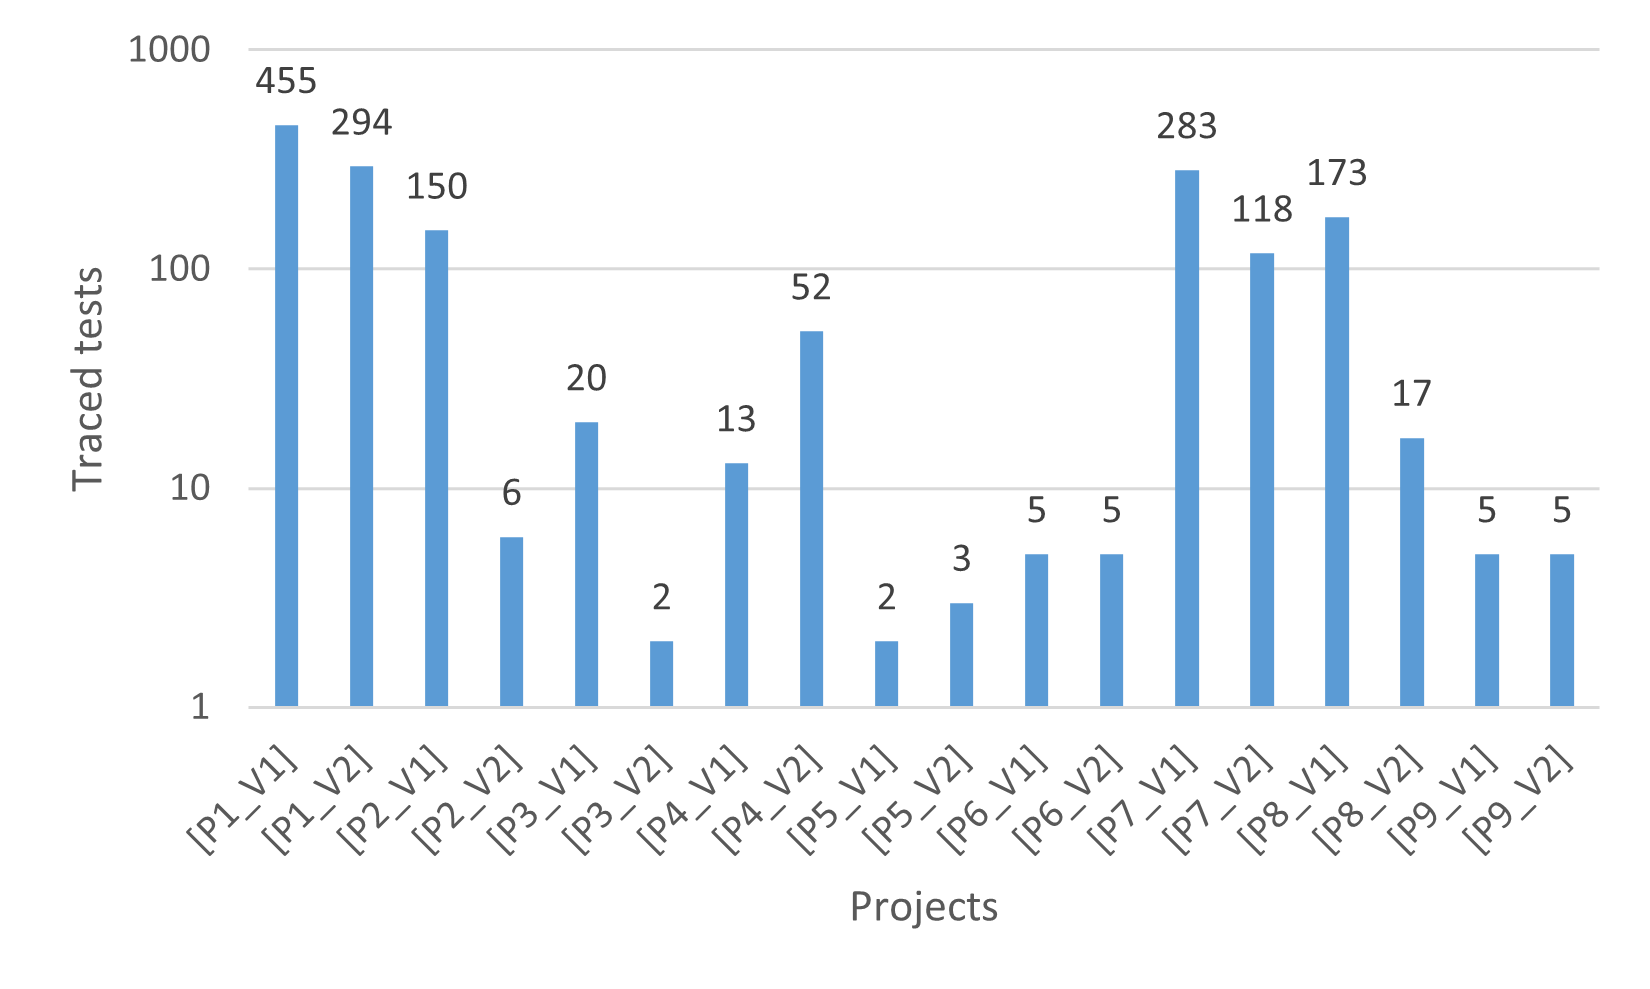
\includegraphics[width=0.75\textwidth]{./pics/chapter2pics/tracedTests1.png}
	%\vspace{-1em}
	\caption{\red{Traced tests due to metamodel evolution in each project.}}
	\label{fig:tracedTests}
	%\vspace{-5mm}
\end{figure}

\begin{tcolorbox}[boxsep=-2pt]
	\textbf{$\boldsymbol{RQ_1}$ insights:}
	We could successfully trace the tests that must be executed before and after the co-evolution regardless of whether they are manually or automatically written. This would help developers to immediately check the code co-evolution by executing the subset of relevant traced tests among the whole test suite. 
\end{tcolorbox}

\subsubsection{RQ2. What is the observed behavioral correctness level of the code co-evolution?}

After tracing the tests, we could execute them to observe their effect before and after co-evolution of the code. Table \ref{table:tracedTests} depicts the results for the original and evolved projects' versions. The second line gives the number of traced class tests and the rest of the lines categorizes the tests. \red{We overall observe no significant difference between projects with automatically generated tests and projects with manually tests.} 

The most interesting project is the first $[P1_{V1}]$ to $[P1_{V2}]$. Even though the tests decreased by \red{161 (455 - 294 from Figure \ref{fig:tracedTests}}), the number of passing tests decreased only by 9 (\red{106 - 97 from Table \ref{table:tracedTests}}). Regarding the error tests, they decreased by 155. However, the failing tests increased by 3 from 2 to 5\red{, as shown in Table \ref{table:tracedTests}. There was also the appearance of one failing test in $[P8]$.} These cases of increased failing tests indicate that the code co-evolution may be not completely behaviorally correct. 

Moreover, in the other projects $[P2][P3][P7][P8]$, many tests that existed in the original version were not in the evolved version due to the delete changes of the metamodels. This is actually a sign of behavioral correct co-evolution, as indeed the tests should be removed following the removal of the generated code for those deleted metamodel elements. 
\red{}In the rest of the projects $[P4][P5][P6][P9]$, roughly the same number of tests in the original version behaved the same in the evolved version, suggesting again a behaviorally correct co-evolution.
These results should help developers to further check the code co-evolution rather than simply accepting them in particular when it is fully automated. 

%\red{chech the three categrories of tests exists: 1/ in V1 and not in V2, 2/ in V1 and V2, 3/ in V2 and not V1.}

\begin{table*}[t]
	%\begin{wraptable*}{r}{5.5cm}
	\centering
	\caption{Selected tests before and after code co-evolution.} %[Legend: Before (V1) -- After (V2) ]}
\label{table:tracedTests}
%
%\small
%\hspace*{-2em}
\resizebox{13cm}{!}{
	\begin{tabular}{
			@{\hskip3pt}c@{\hskip3pt}|c@{\hskip3pt}|c@{\hskip3pt}|c@{\hskip3pt}|c@{\hskip3pt}|c@{\hskip3pt}|c@{\hskip3pt}|c@{\hskip3pt}|| c@{\hskip3pt} |c@{\hskip3pt} }
		\toprule 
		Projects
		& \begin{tabular}[c]{@{}l@{}}$[P1_{V1}]$ \\ to \\$[P1_{V2}]$\end{tabular}
		& \begin{tabular}[c]{@{}l@{}}$[P2_{V1}]$ \\to \\$[P2_{V2}]$\end{tabular} &\begin{tabular}[c]{@{}l@{}} $[P3_{V1}]$ \\to\\ $[P3_{V2}]$ \end{tabular}
		&\begin{tabular}[c]{@{}l@{}} $[P4_{V1}]$ \\to \\$[P4_{V2}]$\end{tabular}
		&\begin{tabular}[c]{@{}l@{}} $[P5_{V1}]$\\ to\\ $[P5_{V2}]$\end{tabular}
		& \begin{tabular}[c]{@{}l@{}}$[P6_{V1}]$ \\to\\ $[P6_{V2}]$\end{tabular} 
		& \begin{tabular}[c]{@{}l@{}}$[P7_{V1}]$ \\to\\ $[P7_{V2}]$\end{tabular}
		&\begin{tabular}[c]{@{}l@{}}$[P8_{V1}]$ \\to\\ $[P8_{V2}]$\end{tabular}
		&\begin{tabular}[c]{@{}l@{}}$[P9_{V1}]$ \\to\\ $[P9_{V2}]$\end{tabular}\\ \midrule%{2-10}
		
		
		\begin{tabular}[c]{@{}l@{}}$N^{o}$ class\\ tests \end{tabular} &  114 - 57 &  51 - 4   &   8 - 2  &  5 - 10   &   2 - 3   &   2 - 3   &   11 - 12  &   32 - 8  &   1 - 1    \\ \midrule \midrule
		
		
		\begin{tabular}[c]{@{}l@{}}$N^{o}$ \\ pass\end{tabular} & \begin{tabular}[c]{@{}l@{}} 106 - 97 \end{tabular} & \begin{tabular}[c]{@{}l@{}}  124 - 0  \end{tabular} &\begin{tabular}[c]{@{}l@{}}  14 - 1  \end{tabular}  
		&\begin{tabular}[c]{@{}l@{}}  10 - 22  \end{tabular}  
		&\begin{tabular}[c]{@{}l@{}}  2 - 3 \end{tabular}  &
		\begin{tabular}[c]{@{}l@{}}2 - 2\end{tabular} & \begin{tabular}[c]{@{}l@{}}206 - 68\end{tabular}
		& \begin{tabular}[c]{@{}l@{}}146 - 10\end{tabular}
		& \begin{tabular}[c]{@{}l@{}}5 - 5 \end{tabular}\\ \midrule
		
		
		\begin{tabular}[c]{@{}l@{}}$N^{o}$\\ fail\end{tabular} & \begin{tabular}[c]{@{}l@{}} 2 - 5  \end{tabular} & \begin{tabular}[c]{@{}l@{}}  1 - 1  \end{tabular} &\begin{tabular}[c]{@{}l@{}}  0 - 0  \end{tabular}  
		&\begin{tabular}[c]{@{}l@{}}  1 - 3  \end{tabular}  
		&\begin{tabular}[c]{@{}l@{}}  0 - 0 \end{tabular}  
		&\begin{tabular}[c]{@{}l@{}}0 - 0 \end{tabular}  & \begin{tabular}[c]{@{}l@{}}1 - 0\end{tabular}
		&\begin{tabular}[c]{@{}l@{}}0 - 1 \end{tabular} 
		&\begin{tabular}[c]{@{}l@{}}0 - 0\end{tabular} 
		\\ \midrule
		
		
		\begin{tabular}[c]{@{}l@{}}$N^{o}$\\ error\end{tabular} & \begin{tabular}[c]{@{}l@{}} 347 - 192 \end{tabular} & \begin{tabular}[c]{@{}l@{}}  25 - 5\end{tabular} &\begin{tabular}[c]{@{}l@{}}  6 - 1  \end{tabular}   
		&\begin{tabular}[c]{@{}l@{}}  2 - 27  \end{tabular}  
		&\begin{tabular}[c]{@{}l@{}}  0 - 0  \end{tabular}  &
		\begin{tabular}[c]{@{}l@{}} 3 - 3  \end{tabular}  & \begin{tabular}[c]{@{}l@{}}76 - 50\end{tabular}
		& \begin{tabular}[c]{@{}l@{}}27 - 6\end{tabular} 
		& \begin{tabular}[c]{@{}l@{}}0 - 0\end{tabular} \\ 
		
		
		\bottomrule
	\end{tabular}
}
%\end{wraptable*} 
%\vspace{-1em}
\end{table*}

\begin{tcolorbox}[boxsep=-2pt]
\textbf{$\boldsymbol{RQ_2}$ insights:}
Our traced tests could hint in two projects that the co-evolution may not be entirely correct due to more failing tests and fewer passing tests. The rest of the project would hint on rather a correct co-evolution due to delete metamodel changes. Overall, automating the help for checking of the behavioral correctness of the code co-evolution for developers, regardless of whether they tests are manually or automatically written.  
\end{tcolorbox}



\subsubsection{RQ3. What are the observed gains (w.r.t. test case reduction and execution time) obtained from our approach of tracing impacted tests by metamodel evolution ?}
With the traced tests due to the metamodel evolution, we can assess the gains in terms of test reduction and execution time compared to the whole test suite as a baseline. 
Indeed, rather than re-running the whole test suite both in the original and evolved versions, or worse, not considering the tests at all. We provide developers with a zoomed view of traced impacted tests by the metamodel evolution, hence, focusing on assessing the code co-evolution.  

The first line of Table \ref{table:tracedTests} already gives the number of traced impacted test classes that are always less than the original number of test classes. 

Table \ref{CaseStudies_CoEvolution_result} further illustrates the differences between the original test suite and the traced impacted tests in terms of number of test cases and execution time. Columns~2 and~3 give the number of original tests and of traced tests.
%
%Figure \ref{fig:testReduction} 
Column 4 depicts the gains in terms of test reduction percentage. On average, we observe a reduction gain of~88\% of test cases, varying from 46\% to 99.9\%. Out of 34612 tests in the 18 projects, we traced 1608 impacted tests representing an absolute 95\% reduction.

This naturally leads to a gain in terms of execution time reduction of the tests. 
Columns 5 and 6 give the execution times for the whole test cases and the traced ones. Herein, we measured the execution time through IDE runner for the Junit tests.
%Figure \ref{fig:testReduction}
Column 7 depicts the gains in execution time of the traced tests compared to the whole test suite. On average, we observe a reduction of 84\%, varying from 69\% to 99\%. 
%84.6\%
\red{Overall, we observe no significant difference in benefit of reducing tests and the gain in execution time between projects with automatically generated tests and projects with manually tests. Respectively, we observe a reduction gain in tests of 88\% versus~81\% and a reduction gain in execution of 82\% versus 95.5\%.} 


%\begin{table*}[t]
\begin{sidewaystable}
\centering
\caption{Reduction gains of the number of traced tests and their execution time.}
\label{CaseStudies_CoEvolution_result}
%\hspace*{-4em}
\resizebox{22cm}{!} {
	\begin{tabular}{lcccccc}
		\toprule
		\begin{tabular}[c]{@{}l@{}}Projects co-evolved in response to the evolved \\ metamodels \end{tabular} 
		& \begin{tabular}[c]{@{}c@{}}$N^{o}$ of \\ tests\end{tabular}
		& \begin{tabular}[c]{@{}c@{}}$N^{o}$ of \\ traced tests\end{tabular}
		&  \begin{tabular}[c]{@{}c@{}}Reduction \\ gain \\ in tests \end{tabular}
		& \begin{tabular}[c]{@{}c@{}}Execution \\ time of \\ tests (s)\end{tabular} 
		&\begin{tabular}[c]{@{}c@{}}Execution \\ time of \\ traced tests (s)\end{tabular}
		&\begin{tabular}[c]{@{}c@{}}Reduction \\gain in \\ execution time \end{tabular} %& \begin{tabular}[c]{@{}c@{}}$N^{o}$ of total \\ direct errors \end{tabular}& \begin{tabular}[c]{@{}c@{}}$N^{o}$ of total \\ indirect errors \end{tabular}
		\\ \midrule		
		
		$[P1_{V1}]$ ocl.examples.pivot & 7322 & 455
		&  \cellcolor{green!40}$\searrow$ 94\% &339.411  & 48.322 & \cellcolor{green!35}$\searrow$ 86\% \\ \midrule
		
		$[P1_{V2}]$ ocl.examples.pivot & 4990 & 294 & \cellcolor{green!40}$\searrow$ 94\%  & 228.88  & 70.856 & \cellcolor{green!25}$\searrow$ 69\% \\ \midrule
		
		$[P2_{V1}]$ ocl.examples.base & 2320 & 150 & \cellcolor{green!40}$\searrow$ 93.5\%  & 123.254 & 26.518& \cellcolor{green!30}$\searrow$ 79\% \\ \midrule
		
		$[P2_{V2}]$ ocl.examples.base & 2133 & 6 & \cellcolor{green!40}$\searrow$ 99.7\%  & 99.105 & 5.294 & \cellcolor{green!40}$\searrow$ 95\% \\ \midrule
		
		
		$[P3_{V1}]$ ocl.pivot & 8795 & 20 & \cellcolor{green!40}$\searrow$ 99.7\%  &859.69 &  0.497& \cellcolor{green!40}$\searrow$ 99\% \\ \midrule
		
		$[P3_{V2}]$ ocl.pivot & 6396 & 2 & \cellcolor{green!40}$\searrow$ 99.9\%  & 261.792 & 12.133 & \cellcolor{green!40}$\searrow$ 95\% \\ \midrule
		
		$[P4_{V1}]$ papyrus.infra.extendedtypes & 135 & 13 & \cellcolor{green!40}$\searrow$ 90\%  &16.94 &  2.924& \cellcolor{green!35}$\searrow$ 83\% \\ \midrule
		
		$[P4_{V2}]$ papyrus.infra.extendedtypes & 248 & 52 & \cellcolor{green!30}$\searrow$ 79\%  & 17.076 & 2.957& \cellcolor{green!35}$\searrow$ 83\% \\\midrule
		
		$[P5_{V1}]$ papyrus.infra.extendedtypes.emf & 104 & 2 & \cellcolor{green!40}$\searrow$ 98\%  & 6.912& 2.11& \cellcolor{green!25}$\searrow$ 70\% \\ \midrule
		$[P5_{V2}]$ papyrus.infra.extendedtypes.emf & 104 & 3  & \cellcolor{green!40}$\searrow$ 97\%  & 7.31& 1.802 & \cellcolor{green!25}$\searrow$ 75\% \\ \midrule
		
		$[P6_{V1}]$ papyrus.uml.tools.extendedtypes & 75 & 5 & \cellcolor{green!40}$\searrow$ 93\%  &5.9 & 1.505 & \cellcolor{green!25}$\searrow$ 75\% \\ \midrule
		
		$[P6_{V2}]$ papyrus.uml.tools.extendedtypes & 75 & 5 &  \cellcolor{green!40}$\searrow$ 93\% & 6.246 & 1.099& \cellcolor{green!35}$\searrow$ 82\% \\ \midrule
		
		$[P7_{V1}]$ org.eclipse.modisco.infra.discovery.benchmark& 524 & 283 & \cellcolor{green!10}$\searrow$ 46\%  & 7.332 & 2.04 & \cellcolor{green!25}$\searrow$ 73\%  \\ \midrule
		
		$[P7_{V2}]$ org.eclipse.modisco.infra.discovery.benchmark& 619 & 118 & \cellcolor{green!35}$\searrow$ 81\%  & 14.534 &4.107  & \cellcolor{green!25}$\searrow$ 72\% \\% \midrule
		\midrule
		
		$[P8_{V1}]$ org.eclipse.emf.test.core& 322 & 173 & \cellcolor{green!10}$\searrow$ 46\%  & 176.372 & 2.908 & \cellcolor{green!40}$\searrow$ 98\%  \\ 
		\midrule
		
		$[P8_{V2}]$ org.eclipse.emf.test.core& 322 & 17 & \cellcolor{green!40}$\searrow$ 94\%  & 157.041& 0.346 & \cellcolor{green!40}$\searrow$ 99\%  \\ 
		
		\midrule
		
		$[P9_{V1}]$ org.eclipse.emf.test.xml& 64 & 5 & \cellcolor{green!40}$\searrow$ 92\%  & 3.764 & 0.247 & \cellcolor{green!40}$\searrow$ 93\%  \\ 
		\midrule
		
		$[P9_{V2}]$ org.eclipse.emf.test.xml& 64 & 5 & \cellcolor{green!40}$\searrow$ 92\%  & 3.193 & 0.257 & \cellcolor{green!40}$\searrow$ 92\%  \\ 
		
		
		
		\bottomrule		
	\end{tabular}
	%}
}
%\end{table*}
\end{sidewaystable}
\begin{comment}

\begin{figure}[t]
	\centering
	%\hspace*{-2em}
	\includegraphics[width=0.5\textwidth]{img/.png}
	%\vspace{-1em}
	\caption{Reduction gains of traced tests from the whole test suite in each project.}
	\label{fig:gain1}
	%\vspace{-5mm}
\end{figure}

\begin{figure}[t]
	\centering
	%\hspace*{-2em}
	\includegraphics[width=0.5\textwidth]{img/.png}
	%\vspace{-1em}
	\caption{Execution gains of traced tests from the whole test suite in each project.}
	\label{fig:gain2}
	%\vspace{-5mm}
\end{figure}
\end{comment}


\begin{tcolorbox}[boxsep=-2pt]
\textbf{$\boldsymbol{RQ_3}$ insights:}
Tracing the metamodel evolution changes up to the impacted tests allows assessing the co-evolution behavioral correctness, while %Doing so, our approach gains represent
gaining, on average, a reduction of 88\% in the number of tests and 84\% in execution time. The reduction gains are similar with no significant difference regardless of whether the tests are manually or automatically written.
\end{tcolorbox}




\section{Threats to Validity}\label{threat}
\noindent This section discusses threats to validity \cite{wohlin2012experimentation}.

\subsection{Internal Validity.}
To be able to trace the impact of metamodel changes to the tests, we had to have a test suite in the selected projects. However, we observed that the Eclipse projects relying on metamodels do not come with the test suite. This was not only the case of OCL\cite{MDTOCL}, papyrus \cite{MDTPapyrus} or Modisco \cite{MDTModisco}, but also other Eclipse languages \cite{UML241,BPMN2}. Therefore, we were obliged to generate the test suite with a state-of-the-art available tool EvoSuite \cite{fraser2011evosuite}. 
Even though, automatic test generation is a best practice, there is the risk of having tests that are different from manually written tests. 
However, this does not pose a risk to our approach as the main algorithm of our approach is generic and would be able to trace the impact of a metamodel change in the same way for both automatically generated tests as well as manually written tests. \red{This is what we observed with the fourth EMF case study having manually written tests. Indeed, the overall results of tracing tests and reduction gains were not significantly different in all case studies regardless of whether the tests are automatically generated or manually written.} 
The main risk is related to the behavioral correctness of the code co-evolution. To check it, we require unit tests that target single methods. 
However, automatic test generation can even be more advantageous herein. Indeed, it generates tests for all public methods, whereas developers tend to manually write only few tests for some targeted methods. Thus, if relying only on manually written tests, there is a high risk of not assessing the behavioral correctness of many cases of code co-evolutions that are not covered by test cases. 
This is mitigated by relying on EvoSuite that generates a full test suite of unit tests with Junit assertions. This tool has shown his efficiency in test generation as a state-of-the-art tool~\cite{DANGLOT2019110398,https://doi.org/10.1002/stvr.1601}. \red{Indeed, this is observed when computing the coverage metric for each of our considered projects (see Table \ref{table:coverage}). The highest coverage is on projects with automatically generated tests and the lowest coverage is on the two projects with manually written tests.}

Therefore, our approach not only checks the correctness of the code co-evolution with the traced tests, but also favors the best practice of tests generation in each release of a software language after its metamodel evolution.
%\red{Furthermore, as we studied releases, there is a risk that a test verdict is not only impacted by a code co-evolution but also by other code changes. This, is why we provide a diagnostic for developers with the traced tests as starting point to investigate. Nonetheless, if our approach is performed in a continuous integration mode after each code co-evolution, the traced tests verdicts will solely be due to the given metamodel change.} 

Finally, as our tracing approach relies on the quality of detected metamodel changes, we analyzed, in our evaluation, each detected change and checked whether it occurred between the original and evolved metamodels. This alleviates the risk of relying on an incorrect metamodel change that would degrade the tracing of the impacted tests by metamodel changes, i.e., not tracing an impacted test by a non-considered metamodel change. 
%we plan to run an experiment with devolopers
\red{In addition, as we did not have the ground truth, we could not report on the precision and recall of our approach. 
However, our approach uses the Code Call Graph and starts from the generated code elements corresponding to the evolved metamodel elements to recursively trace back any existing tests. Thus, by design we actually detect all the impacted tests that must be traced. To test that our algorithm does not miss any impacted test, and does not trace non-impacted tests, we manually verified the ground truth for our smallest data set projects $[P6]$ and $[P9]$, because they have fewer tests and are less complex. We checked for every metamodel change all the impacted tests and we found that our approach traces all of them. 
Further evaluation on a ground truth is left for future work.} 

\subsection{External Validity.} 
We implemented and evaluated our approach for EMF/Ecore metamodels and Java code with Junit tests. Other languages, such as C\# or C++, use a different syntax, but conceptually use the same constructions as in Java.
Although we think that the tracing would be applicable for other languages, we cannot generalize our results. Further experimentation on other languages is necessary. However, the only requirement to apply our approach to other languages is to have access to the ASTs of the parsed code and tests, and to adapt our tracing of the tests in the build call graph. 
%
Moreover, our evaluation was performed on Eclipse projects from five languages. Thus, we cannot generalize our findings to all software languages or DSLs. We also cannot generalize our results on manually written tests, in particular the test verdicts of the traced tests, i.e., pass, fail, and error. Further experimentation remains necessary and is left for future work. 

\subsection{Conclusion Validity.}
Our evaluation gave promising results, showing that we could trace the impact of metamodel changes till the tests, and hence, check the behavioral correctness of the code co-evolution in practice for real-world projects. 
However, even though we evaluated our approach on 18 projects of metamodel evolution and code co-evolution with automatically generated tests and manually written tests, further evaluation is needed on more case studies to have more insights and statistical evidence. Finally, our user study experiment suggesting our approach usefulness needs to be replicated with more participants.

\section{Conclusion}
\label{sec_conclusion}
This chapter proposes an automated tracing of the impacted tests due to metamodel evolution. Thus, by tracing the tests before and after code co-evolution, we check its behavioral correctness. 
Our approach takes as input the metamodel changes and then finds the different pattern usages of each metamodel element in the code. 
After that, we recursively search for its usages in the code call graph until reaching the tests. Thus, we end up matching metamodel changes with impacted code methods and their corresponding tests. 
%
We further implemented our approach in an Eclipse plugin that allows to trace the tests, map them with state-of-the-art solution GumTree and execute them. We then report them back as a diagnostic to the developers for an easier in-depth analysis of the effect of metamodel evolutions rather than re-running and analyzing the whole test suite.

The user study experiment we conducted showed that tracing manually the tests impacted by the evolution of the metamodel is a hard and error-prone task. Not only the participants could not trace all tests, but they even wrongly traced non-impacted tests.  
	We then evaluated our approach on 18 Eclipse projects from OCL, Modisco, Papyrus, and EMF over several evolved versions of metamodels. Four projects had manually written tests and we generate tests for the other 14 projects. 
	The results show that we successfully traced the impacted tests automatically by selecting 1608 out of 34612 tests due to 473 metamodel changes. 
	
	%We evaluated our approach on three implementations of OCL, Modisco and Papyrus in Eclipse on 14 projects from over several evolved versions of metamodels, and with generated tests with EvoSuite. Results show that we automatically traced 1408 out of 33840 tests based on the 466 metamodel changes. %928 and 480 impacted tests 
	%
	When running the traced tests before and after co-evolution, we observed two cases indicating possibly both behaviorally incorrect and correct code co-evolution. Thus, helping the developers to locate the code co-evolution to investigate in more detail. Furthermore, our approach provided gains that represent, on average, a reduction of 88\% in number of tests and \red{84\%} in execution time. No significant difference was observed between projects with manually written tests and automatically generated ones.   

%As future work, we first plan to improve the performance of our implementation with optimization of the tests' tracing.  %first evaluate on more case studies that could have manually written test. 
%we will 
%We also plan to extend our approach to projects that use an equivalent form of metamodels in other technological space than Eclipse, such as JHipster and OpenAPI that both generate code from a model specification similar to a metamodel. Thus, we can have alternative case studies. 

%After that, we plan to investigate the techniques of test amplification on the selected tests we traced from the metamodel changes. Indeed, once we select a subset of tests, we could amplify them by generating more similar tests, yet, with different assertions to cover more corner cases. This would amplify the behavioral check of the code co-evolution. 

%Finally, we will also explore another type of amplification, which is the interchange of the tests between the original and evolved versions. In other words, we aim to co-evolve the tests of the original and evolved versions, respectively forward and backward to the evolved and original versions, while removing duplicates. 

%%Moreover, the knowledge about the generated code elements from the metamodel elements (e.g., getter/setter for EAttribute, class/interface for EClass, etc.) is so far hard-coded in the implementation. The mappings must be provided for our approach to be able to trace the tests. We could express these mappings in a generic way as a configuration file taken as input in our approach. Thus, we could reuse our approach more easily in other scenarios than EMF Eclipse (e.g., jHipster), given their corresponding mappings as input. This is left as future work to generalize our approach.


%evaluate existing approaches of automatic code co-evolution with out technique to better assess their effect on the code. 

